\clearpage
\section{Signal extraction using neural networks tools}
\label{signal}
The purpose of the analysis is to search for deviations from the SM predictions in the tW and \ttbar~ production due to new physics, parameterized with the presence of new effective couplings. In order to investigate the effect of the introduction of the new effective couplings,
it is important to find suitable variables with high discrimination power between the signal and the  background.
Depending on the couplings, the total rate (yield) or the distribution of the output of a neural network algorithm (NN) is employed.
The NN algorithm used in this analysis is a multilayer perceptron ~\cite{Denby:1992jd}.


All the effective couplings introduced in Section \ref{tW_Int} can contribute to  tW production except the $O_{G}$ operator.
The introduction of the $O_{G}$ operator affects only the \ttbar~ production. It was shown in Ref. \cite{Cho:1994yu} and checked in this analysis that the top quark transverse momentum distribution is sensitive to the triple gluon field strength operator.
The kinematic distributions of final-state particles show less discrimination power than the  top quark transverse momentum distribution. In addition,  they vary as a function of C$_{G}$ and tend to the SM prediction for decreasing values of the C$_{G}$ coupling. Therefore, we use the total number of events (yield) in  various (n-jets,m-tags) categories to constrain the C$_G$ effective coupling.

The deviation from the SM tW production from the interference terms between the
SM and the $O_{tG}$, $O_{\phi q}^{(3)}$ and $O_{tW}$ operators is of the order of $1/\Lambda^2$.
It is assumed that the new physics scale $\Lambda$ is larger than the scale we probe. Therefore, $1/\Lambda^4$
contributions from the new physics terms are small compared to the contribution from the interference term.
The operator $O_{\phi q}^{(3)}$ is similar to the SM Wtb operator and leads to a rescaling of the SM Wtb vertex.
The $O_{tW}$ and $O_{tG}$ operators provide new interactions compared to the SM Wtb vertex and the top-top-gluon (ttG) vertex.
However, their effects have been investigated through the various kinematic distributions of the final-state particles and are found to be not distinguishable from the SM tW and \ttbar~ processes for unconstrained values of the effective couplings.
After the selection described in Section \ref{tW_Eventselection}, the dominant background comes from the \ttbar~ production, with a contribution of about 90\%.
In order to observe deviations from SM tW production in the presence of the $O_{\phi q}^{(3)}$, $O_{tW}$ and $O_{tG}$ effective operators, we need to separate tW events from the large number of \ttbar~ events.
 Two independent NN are trained to separate \ttbar~ events (the background) and tW events (considered as the signal) in the (1-jet,1-tag) (NN$_{11}$) and (2-jets,1-tag) (NN$_{21}$) categories which have significant signal contributions~\cite{Sirunyan:2018lcp}.
 %A single bin is used for (2-jets,1-tag) category where tW contribution is minimal.



The presence of the $O_{uG}$ and $O_{cG}$ operators changes the initial-state particle (see Figure \ref{fig-feyn}), and leads to different kinematic distributions for the final-state particles, compared to the SM tW process.
For these FCNC operators, new physics effects on final-state particle distributions are expected to be distinguishable from SM processes.
In order to search for new physics due to the $O_{uG}$ and $O_{cG}$ effective operators, a NN (NN$_{\text{FCNC}}$) is used to separate the SM backgrounds (\ttbar~ and tW events together) and the new physics signals for events with exactly one b-tag jet with no requirement on the number of light jets (n-jets,1-tag).

The observables used in the analysis for probing new physics are summarised in Table \ref{NNreg}.
The various input variables for the NN introduced above are shown in Table ~\ref{tab:MVA_var}.


\begin{table}[h]
\caption{Summary of the observables used for probing effective couplings  in various (n-jets,m-tags) categories in the ee and $\mu\mu$ channels.}
\label{NNreg}
\centering
\resizebox{\linewidth}{!}{
\begin{tabular}{|l|l|c|c|c|c|}
\hline
\multirow{2}{*}{Eff. coupling}         & \multirow{2}{*}{Channel}            &  \multicolumn{4}{c|}{Categories } \\ \cline{3-6}
                                       &                                     & 1-jet,1-tag    & 2-jets,1-tag & n-jets,1-tag & $\ge$2-jets,2-tags\\ \hline \hline
\multirow{2}{*}{C$_{G}$}               & ee                                  & Yield          &Yield         &-             &Yield \\
                                       & $\mu\mu$                            & Yield          &Yield         &-             &Yield \\ \hline \hline
\multirow{2}{*}{C$_{\phi q}^{(3)}$, C$_{tW}$, C$_{tG}$ } & ee                &NN$_{11}$       & NN$_{21}$    &-             &Yield \\
                                       & $\mu\mu$                            &NN$_{11}$       & NN$_{21}$    &-             &Yield \\ \hline \hline
\multirow{2}{*}{C$_{uG}$, C$_{cG}$}    & ee                                  &-               &-             &NN$_{\text{FCNC}}$&- \\
                                       & $\mu\mu$                            &-               &-             &NN$_{\text{FCNC}}$&- \\ \hline
\end{tabular}}
\end{table}



\begin{table}[h]
\caption{Input variables for the NN used in the analysis in various  bins of n-jets and m-tags. The symbols ``$\surd$'' indicate the variable
is used.}
\centering
\label{tab:MVA_var}
\small
\smallskip\noindent
\resizebox{\linewidth}{!}{
\begin{tabular}{|l|l|c|c|c|}
\hline                                                                                                                               Variable&    Description      &NN$_{11}$ & NN$_{21}$ &   NN$_{\text{FCNC}}$                  \\ \hline
M$_{ll}$                                                         & Invariant mass of dilepton system                                                    &                          &                 & $\surd$                    \\ \hline
$p_{\text{T}}^{\ell \ell}$                                       & $p_{\text{T}}$ of dilepton system                                                    &                          & $\surd$      & $\surd$                        \\ \hline
$\Delta p_{\text{T}}(\ell,\ell)$                                & $p_{\text{T}}^{\text{leading lepton}}$ - p$_{\text{T}}^{\text{sub-leading lepton}}$   &                          &                 & $\surd$                   \\ \hline
$p_{\text{T}}^{\text{leading lepton}}$                           & $p_{\text{T}}$ of leading lepton                                                     &                          & $\surd$      & $\surd$                       \\ \hline
Centrality($\ell^{\text{leading}}$,jet$^{\text{leading}}$)       & Scalar sum of $p_{\text{T}}$ of the leading lepton and                               & \multirow{2}{*}{}        & \multirow{2}{*}{} & \multirow{2}{*}{$\surd$   }\\
                                                                 & leading jet, over total energy of selected objects                                   &                          &                 &                            \\ \hline
\multirow{2}{*}{Centrality($\ell,\ell$)}                          & Scalar sum of $p_{\text{T}}$ of the leading and sub-leading                         & \multirow{2}{*}{}        & \multirow{2}{*}{} & \multirow{2}{*}{$\surd$   } \\
                                                                 & leptons, over total energy of selected objects                                       &                          &                 &                            \\ \hline
$\Delta \phi(\ell\ell$,jet$^{\text{leading}})$                   & $\Delta \phi$ between dilepton system and leading jet                                & $\surd$              & $\surd$      &\\ \hline
$p_{\text{T}}$($\ell \ell$ ,jet$^{\text{leading}})$              & $p_{\text{T}}$ of dilepton and leading jet system                                    & $\surd$                  &              & $\surd$ \\ \hline
$p_{\text{T}}$($ \ell^{\text{leading}}$,jet$^{\text{leading}})$  & $p_{\text{T}}$ of leading lepton and leading jet system                              & $\surd$                   &             &\\ \hline
\multirow{2}{*}{Centrality($\ell\ell$,jet$^{\text{leading}}$)}   & Scalar sum of $p_{T}$ of the dilepton system and leading                             & \multirow{2}{*}{$\surd$ } & \multirow{2}{*}{} & \multirow{2}{*}{}\\
                                                                 & jet, over total energy of selected objects                                           &                          &                  &\\ \hline
$\Delta$R($\ell,\ell$)                                           & $\Delta$R between leading and sub-leading leptons                                    & $\surd$                  &              & \\ \hline
$\Delta$R($\ell^{\text{leading}}$,jet$^{\text{leading}}$)        & $\Delta$R between leading lepton and leading jet                                     & $\surd$                  &              &\\ \hline
M($\ell^{\text{leading}}$,jet$^{\text{leading}}$)               & Invariant mass of leading lepton and leading jet                                      &                          & $\surd$      & \\  \hline
M(jet$^{\text{leading}}$,jet$^{\text{sub-leading}}$)            & Invariant mass of leading jet and sub-leading jet                                     &                          & $\surd$      & \\ \hline
$\Delta$R($\ell^{\text{leading}}$,jet$^{\text{sub-leading}})$    & $\Delta$R between leading lepton and sub-leading jet                                 &                          & $\surd$      &  \\ \hline
$\Delta$R($\ell \ell$,jet$^{\text{leading}}$)                    & $\Delta$R between dilepton system and leading jet                                    &                          & $\surd$       &  $\surd$   \\ \hline
$\Delta p_{T}(\ell^{\text{sub-leading}}, \text{jet}^{\text{sub-leading}})$ & $p_{\text{T}}^{\text{sub-leading lepton}}$ - $p_{T}^{\text{sub-leading jet}}$    &              & $\surd$      &\\ \hline
M($\ell^{\text{sub-leading}}$, jet$^{\text{leading}}$)               & Invariant mass of sub-leading lepton and leading jet                                   &                          && $\surd$      \\  \hline
\end{tabular}}
\end{table}

The MLP input variables distributions of signal and background events are shown from Figure \ref{fig:input_var_1j1b} to \ref{fig:input_var_FCNC}. The MLP output for test and train samples are shown in Figure \ref{fig:MLP_response}.

\begin{figure}[ht]
  \begin{center}
    \begin{tabular}{c}
      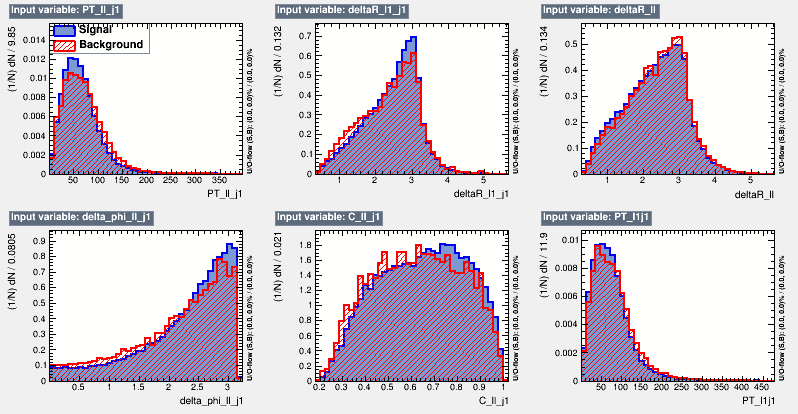
\includegraphics[width=0.82\textwidth]{figures/tW/fig/MVA/MLP_1j1b/var_1.png}\\
    \end{tabular}
    \caption{MLP input variable distributions for NN$_{11}$. Signal distributions are drawn in blue and the background distributions in red.}.
    \label{fig:input_var_1j1b}
  \end{center}
\end{figure}

\begin{figure}[ht]
  \begin{center}
    \begin{tabular}{c}
      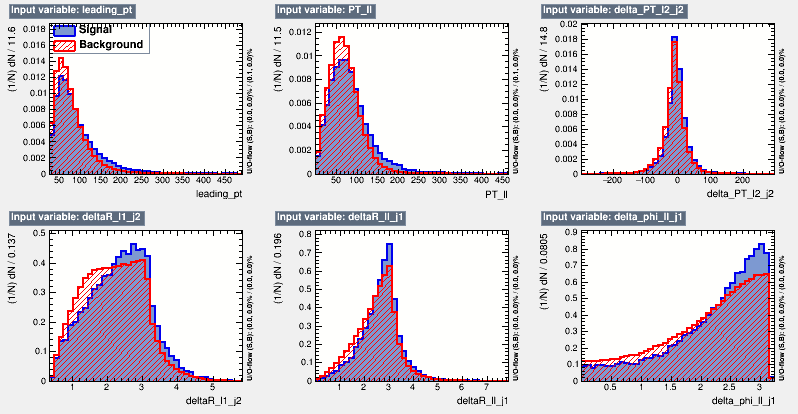
\includegraphics[width=0.82\textwidth]{figures/tW/fig/MVA/MLP_2j1b/var_1.png}\\
      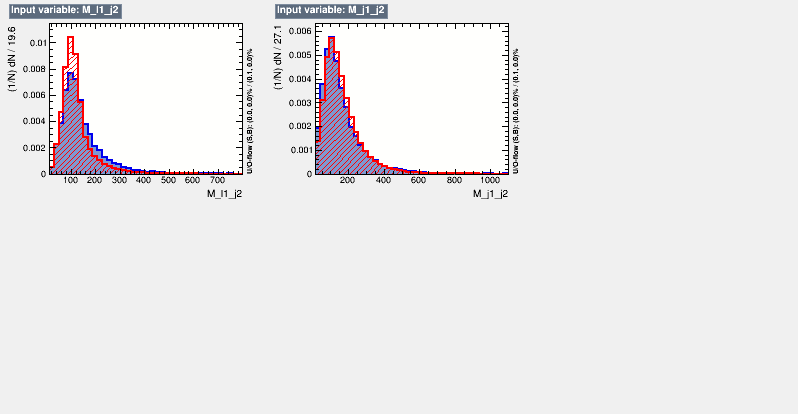
\includegraphics[width=0.82\textwidth]{figures/tW/fig/MVA/MLP_2j1b/var_2.png}\\
    \end{tabular}
    \caption{MLP input variable distributions for NN$_{21}$. Signal distributions are drawn in blue and the background distributions in red.}
    \label{fig:input_var_2j1b}
  \end{center}
\end{figure}

\begin{figure}[ht]
  \begin{center}
    \begin{tabular}{c}
      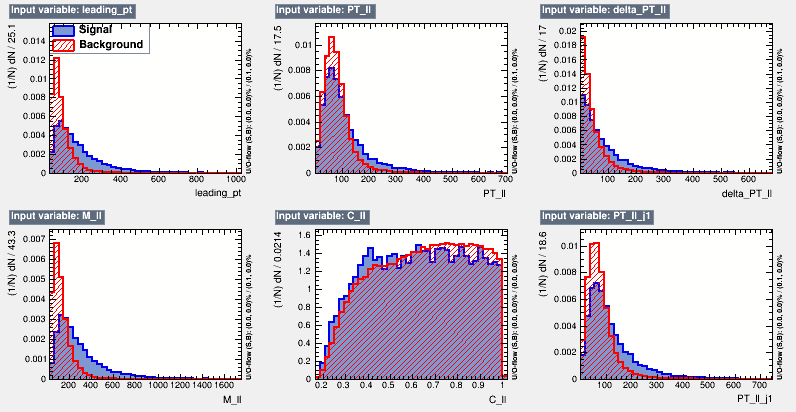
\includegraphics[width=0.82\textwidth]{figures/tW/fig/MVA/MLP_FCNC/var_1.png}\\
      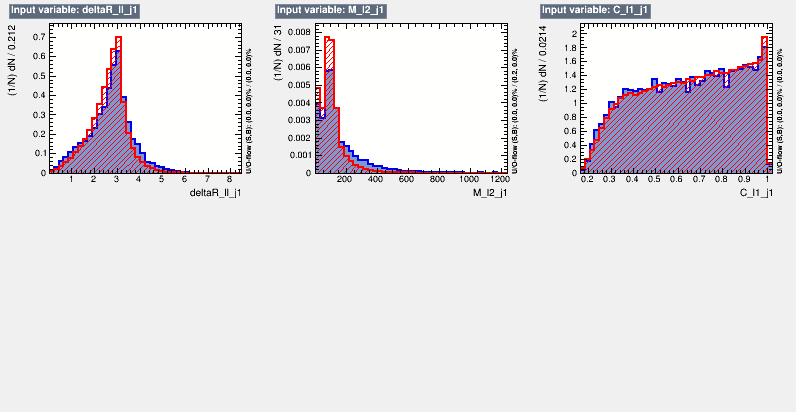
\includegraphics[width=0.82\textwidth]{figures/tW/fig/MVA/MLP_FCNC/var_2.png}\\
    \end{tabular}
    \caption{MLP input variable distributions for NN$_{\text{FCNC}}$. Signal distributions are drawn in blue and the background distributions in red.}
    \label{fig:input_var_FCNC}
  \end{center}
\end{figure}



\begin{figure}[ht]
  \begin{center}
      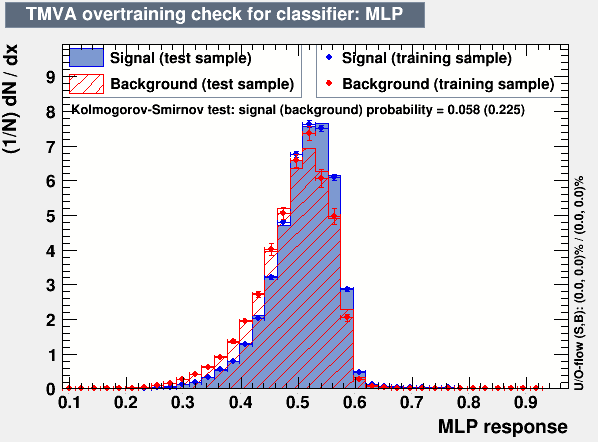
\includegraphics[width=0.6\textwidth]{figures/tW/fig/MVA/MLP_1j1b/MLP.png}
      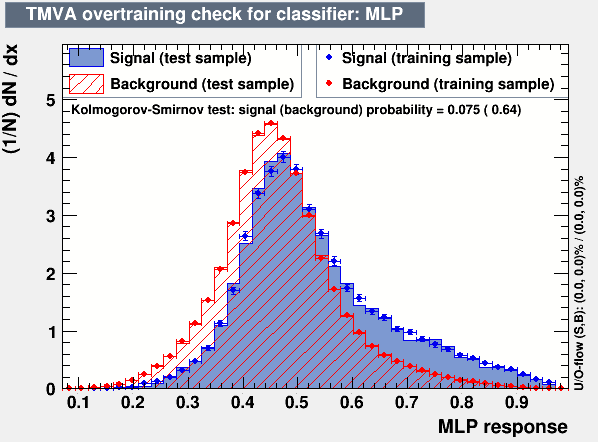
\includegraphics[width=0.6\textwidth]{figures/tW/fig/MVA/MLP_2j1b/MLP.png}
      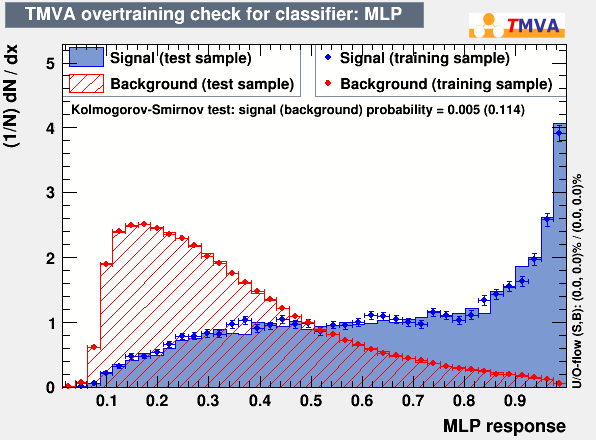
\includegraphics[width=0.6\textwidth]{figures/tW/fig/MVA/MLP_FCNC/MLP.png}
    \caption{MLP output for test and train samples for NN$_{11}$ (top), NN$_{21}$ (middle) and NN$_{\text{FCNC}}$ (bottom) .}
    \label{fig:MLP_response}
  \end{center}
\end{figure}




\subsection{Data/MC comparison for MVA input variables}
\label{MVA_input_variables}
The data and MC comparison for MVA input variables are shown from Figure \ref{fig:MVA_1j1t_1} to \ref{fig:MVA_1j1t_2} for NN$_{11}$, and from Figure \ref{fig:MVA_2j1t_1} to \ref{fig:MVA_2j1t_2} for NN$_{21}$ and from Figure \ref{fig:MVA_FCNC_1j1t_1} to \ref{fig:MVA_FCNC_1j1t_3} for NN$_{\text{FCNC}}$.
Sources of systematic uncertainties which are considered in the plots are explained in Section \ref{tW_systematic}.
Considering the systematic uncertainties, data/MC are in good agreement and no obvious large mis-modelling is observed.


\begin{figure}[ht]
  \begin{center}
    \begin{tabular}{ccc}
      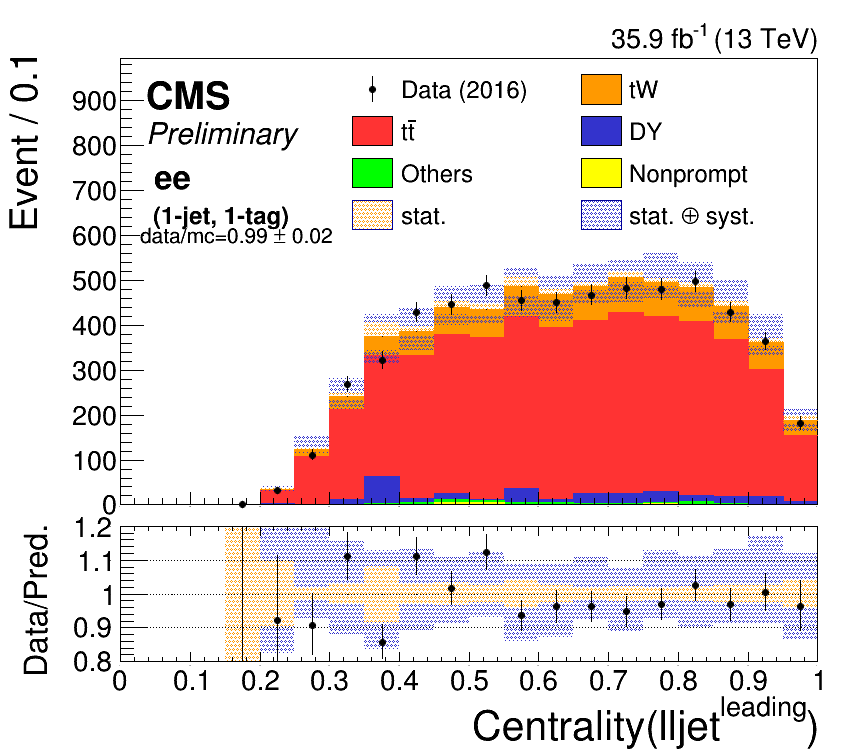
\includegraphics[width=0.4\textwidth]{figures/tW/fig/MVA_input/ee/H_1j1b_Cll_j1.png}&
      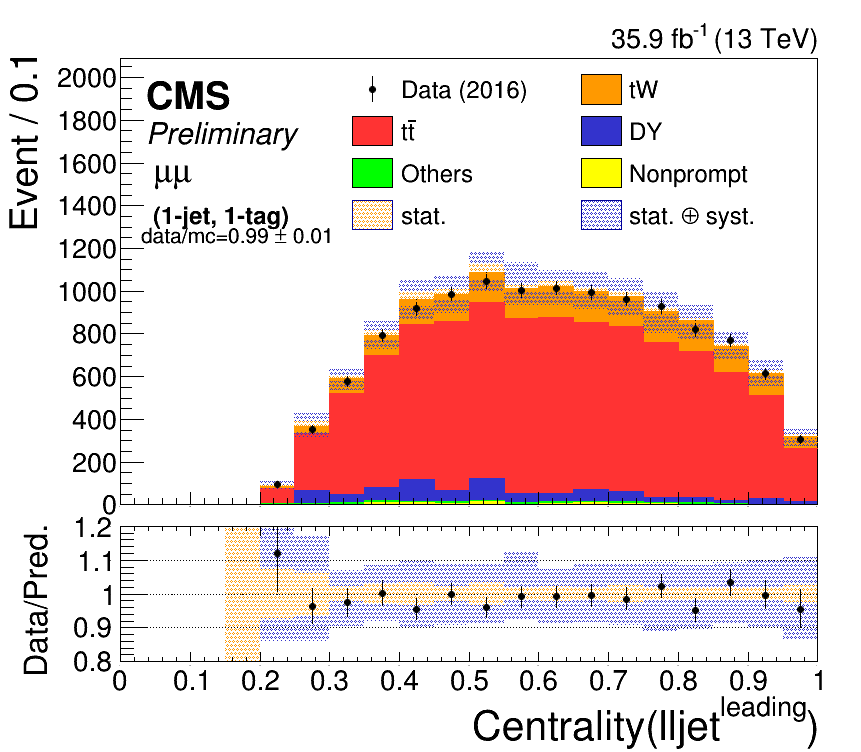
\includegraphics[width=0.4\textwidth]{figures/tW/fig/MVA_input/mumu/H_1j1b_Cll_j1.png}\\
      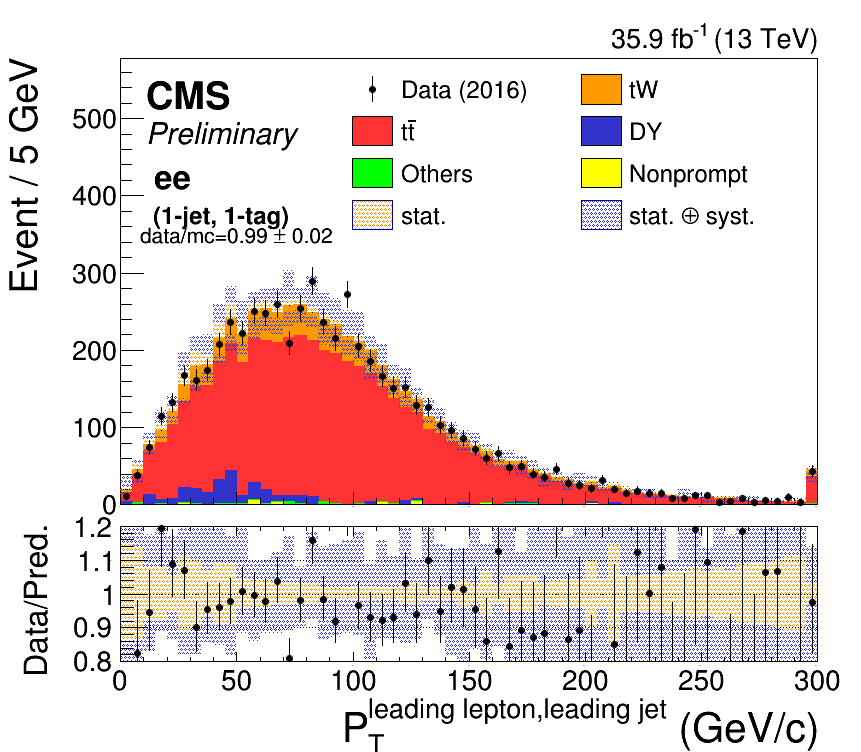
\includegraphics[width=0.4\textwidth]{figures/tW/fig/MVA_input/ee/H_1j1b_l1_j1_pt.png}&
      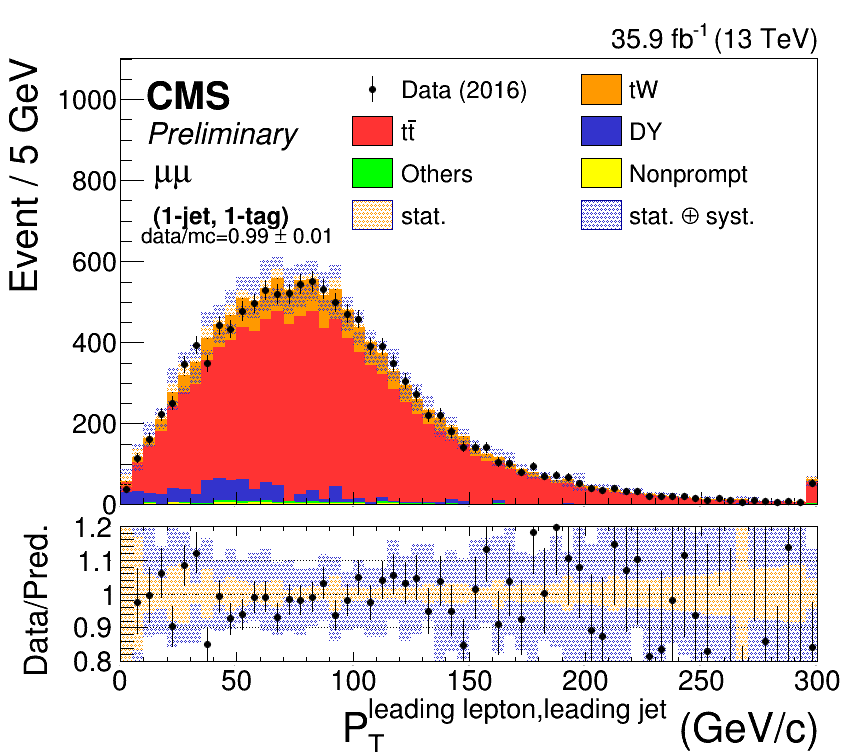
\includegraphics[width=0.4\textwidth]{figures/tW/fig/MVA_input/mumu/H_1j1b_l1_j1_pt.png}\\
      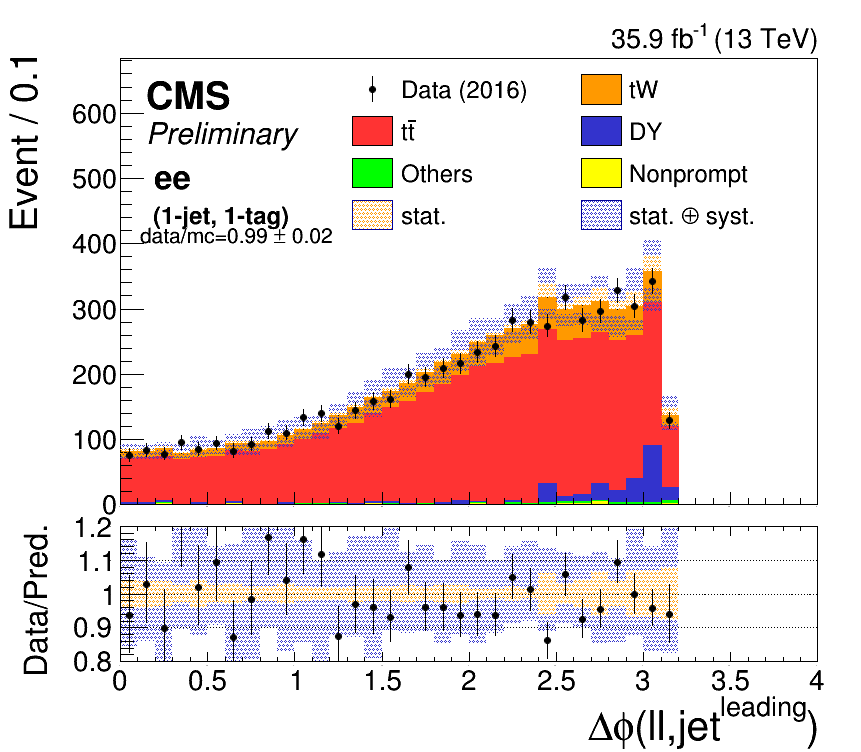
\includegraphics[width=0.4\textwidth]{figures/tW/fig/MVA_input/ee/H_1j1b_dPhi_ll_j1.png}&
      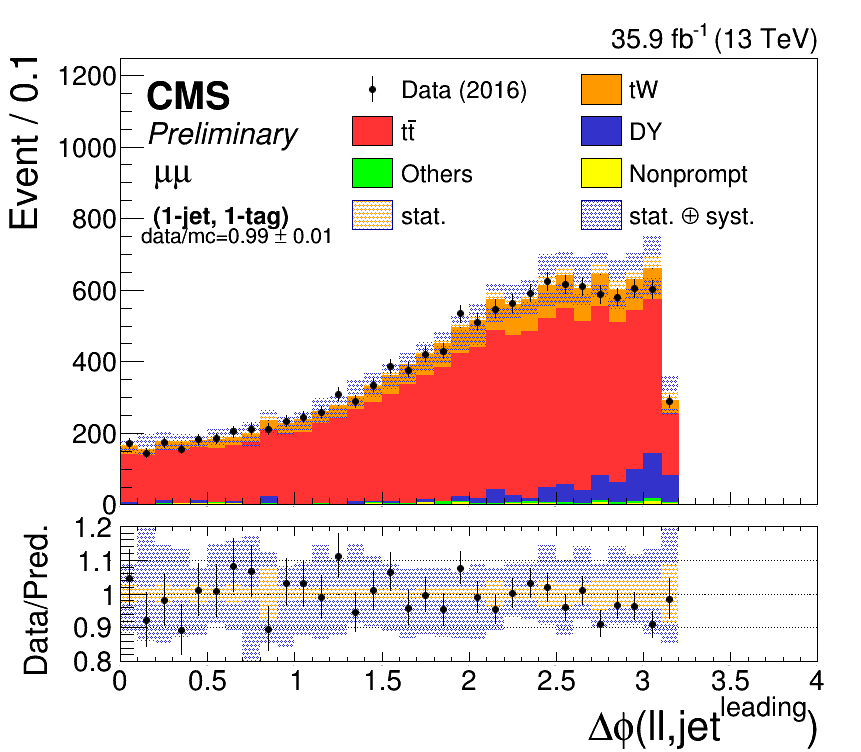
\includegraphics[width=0.4\textwidth]{figures/tW/fig/MVA_input/mumu/H_1j1b_dPhi_ll_j1.png}\\
      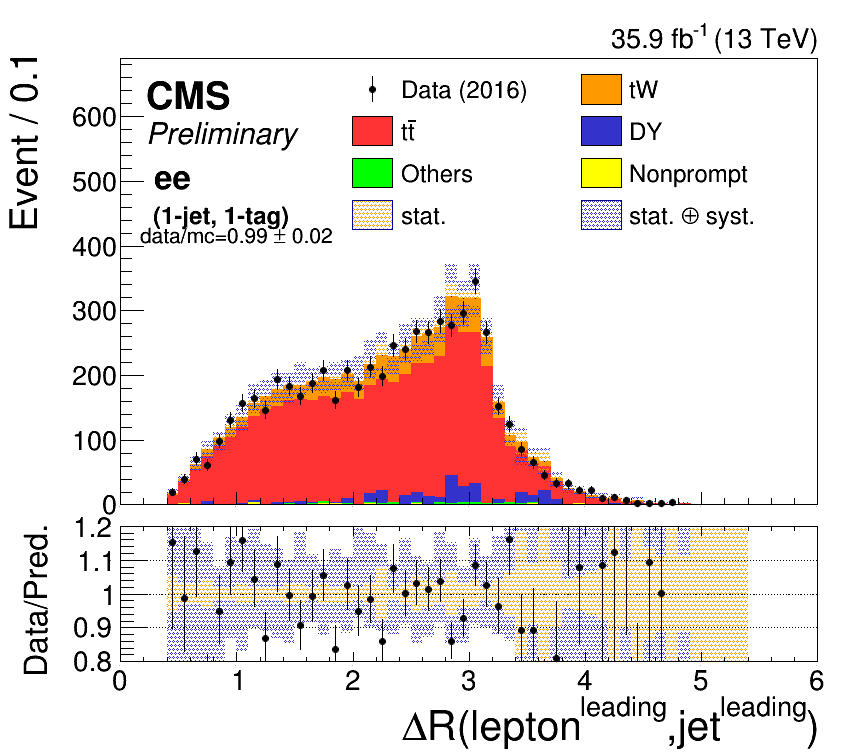
\includegraphics[width=0.4\textwidth]{figures/tW/fig/MVA_input/ee/H_1j1b_dR_l1_j1.png}&
      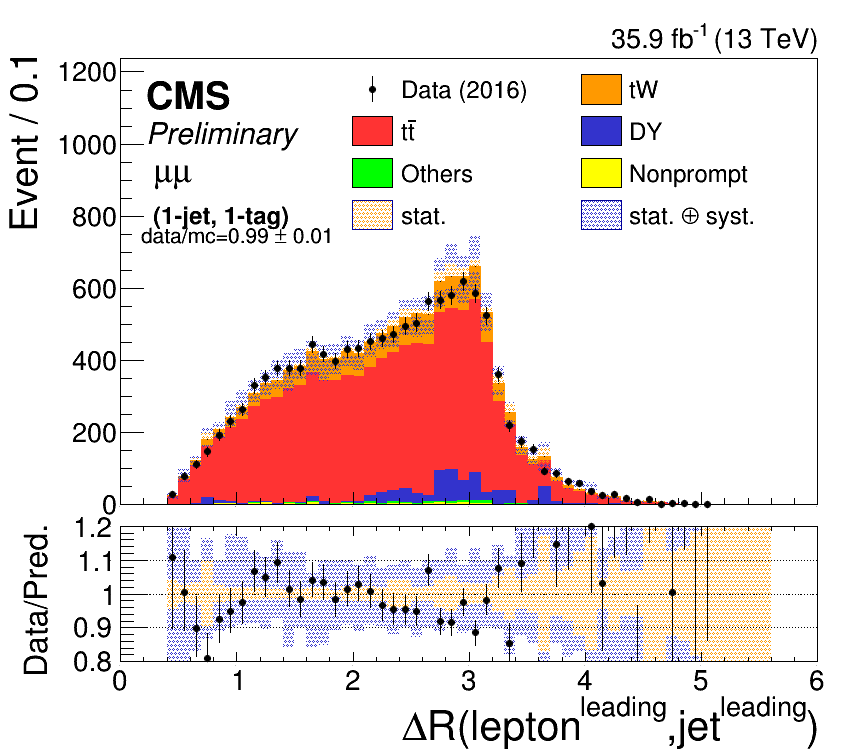
\includegraphics[width=0.4\textwidth]{figures/tW/fig/MVA_input/mumu/H_1j1b_dR_l1_j1.png}\\
    \end{tabular}
    \caption{The distributions of variables used for MVA input for $ee$ (left) and $\mu\mu$ (right) channels for NN$_{11}$.
    \label{fig:MVA_1j1t_1}}
  \end{center}
\end{figure}

\begin{figure}[ht]
  \begin{center}
    \begin{tabular}{ccc}
      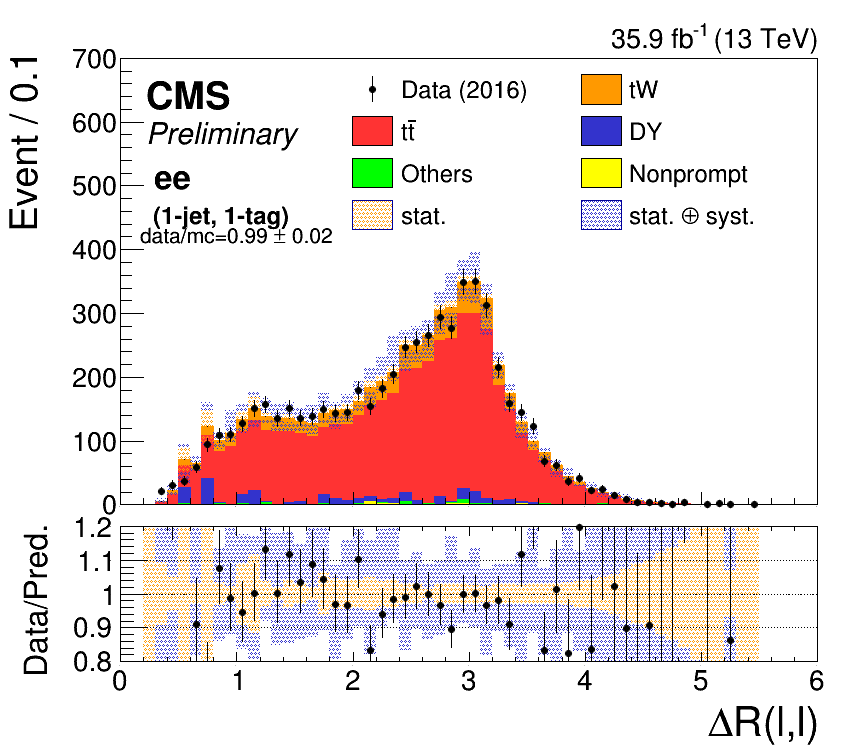
\includegraphics[width=0.4\textwidth]{figures/tW/fig/MVA_input/ee/H_1j1b_dR_l1_l2.png}&
      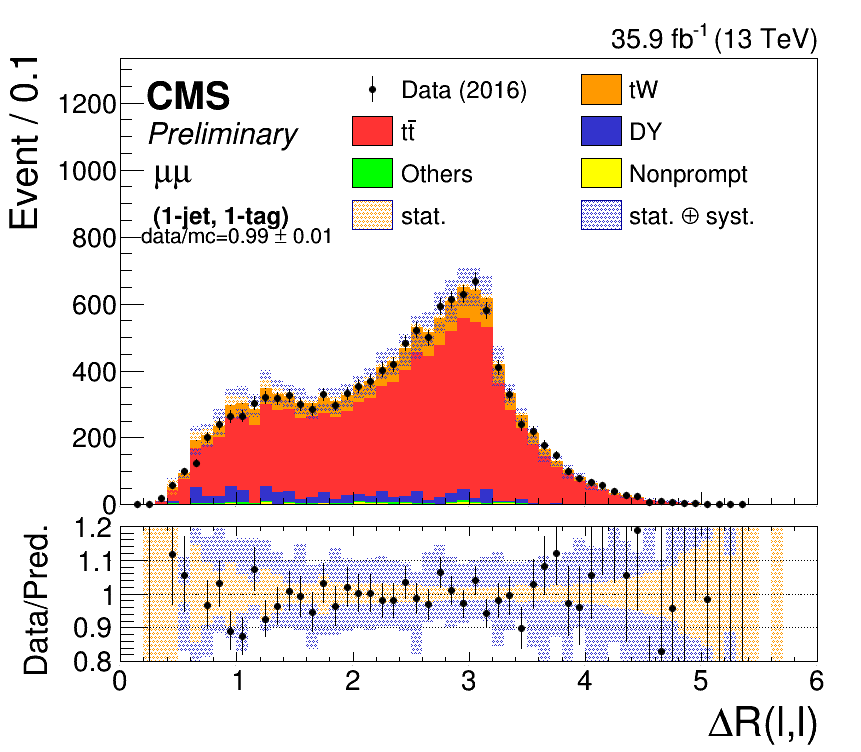
\includegraphics[width=0.4\textwidth]{figures/tW/fig/MVA_input/mumu/H_1j1b_dR_l1_l2.png}\\
      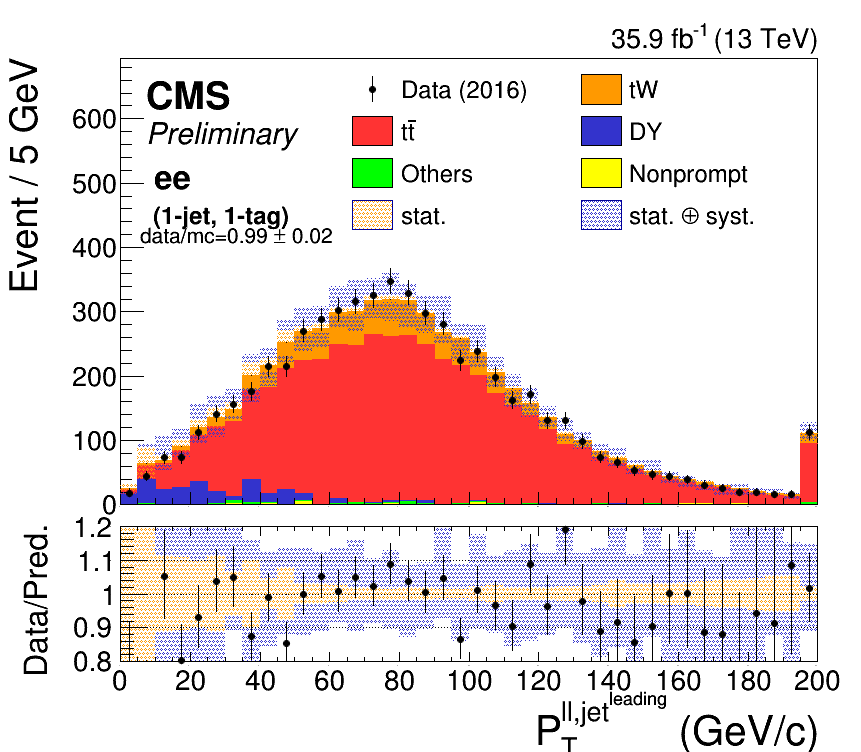
\includegraphics[width=0.4\textwidth]{figures/tW/fig/MVA_input/ee/H_1j1b_ll_j1_pt.png}&
      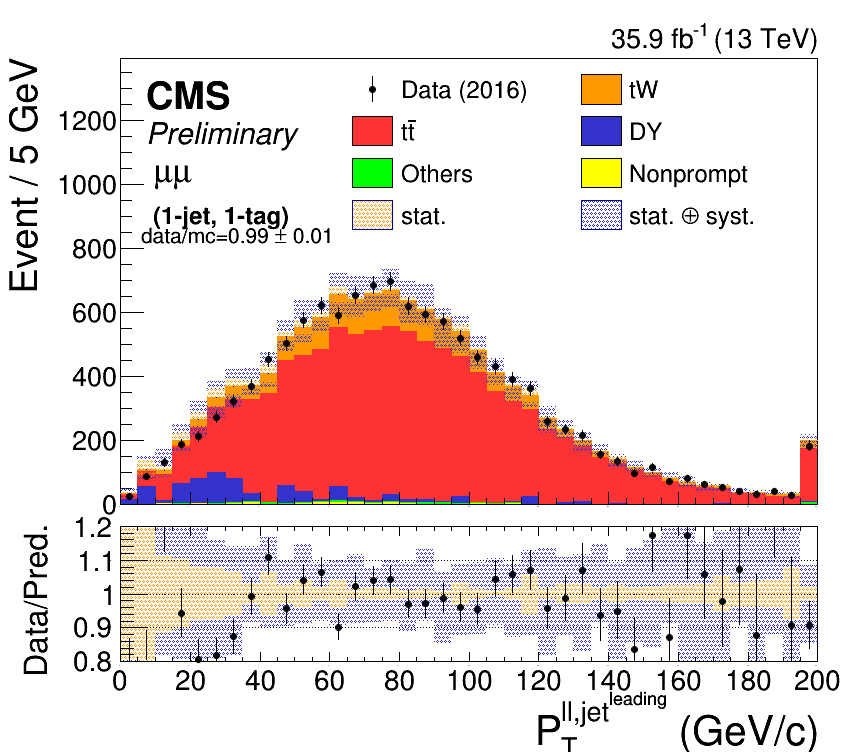
\includegraphics[width=0.4\textwidth]{figures/tW/fig/MVA_input/mumu/H_1j1b_ll_j1_pt.png}\\
    \end{tabular}
    \caption{The distributions of variables used for MVA input for $ee$ (left) and $\mu\mu$ (right) channels for NN$_{11}$.
    \label{fig:MVA_1j1t_2}}
  \end{center}
\end{figure}





\begin{figure}[ht]
  \begin{center}
    \begin{tabular}{ccc}
      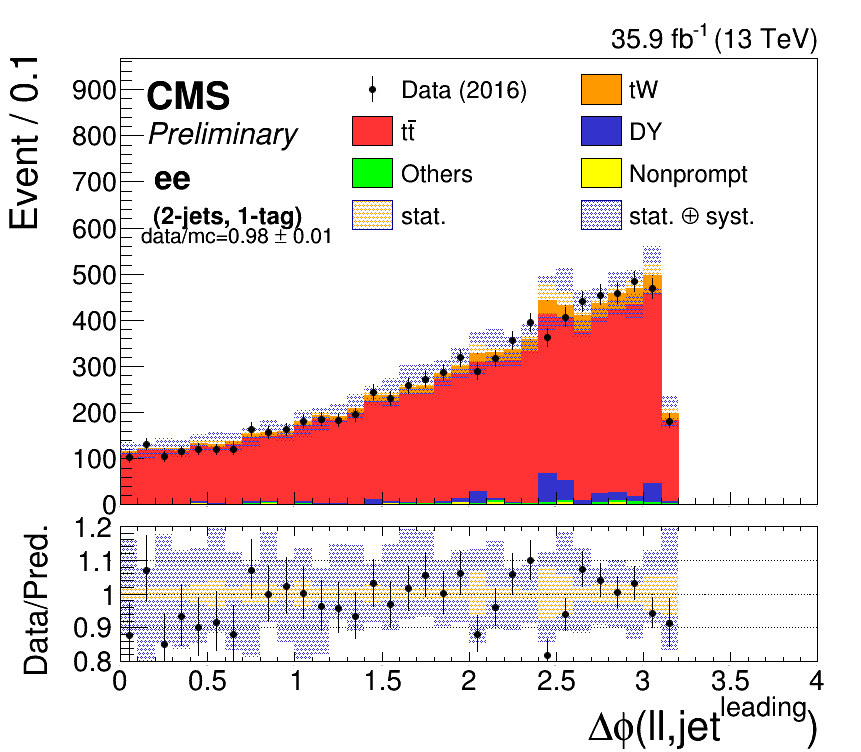
\includegraphics[width=0.4\textwidth]{figures/tW/fig/MVA_input/ee/H_2j1b_dPhi_ll_j1.png}&
      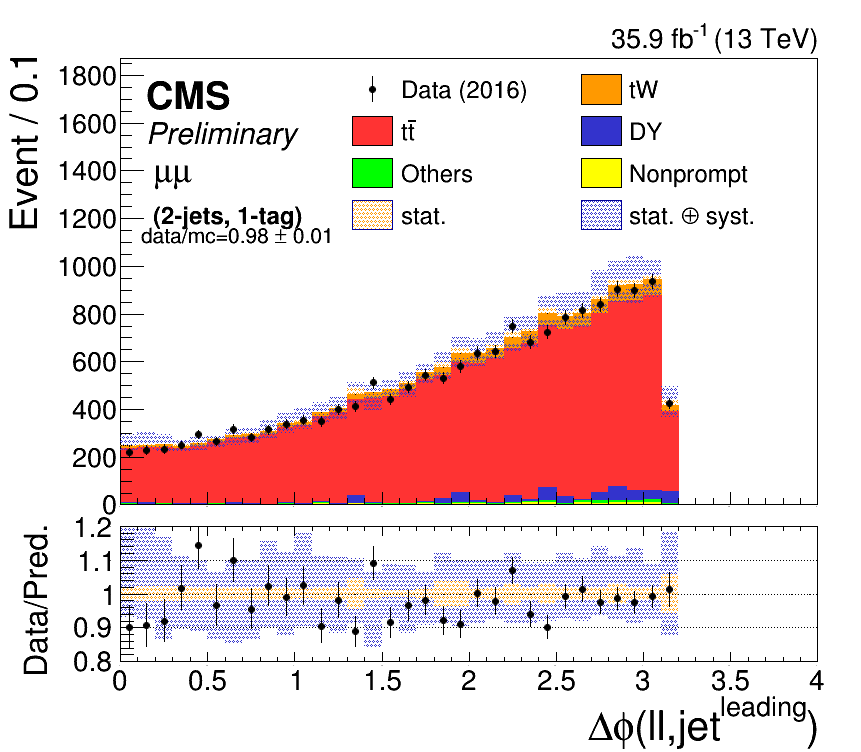
\includegraphics[width=0.4\textwidth]{figures/tW/fig/MVA_input/mumu/H_2j1b_dPhi_ll_j1.png}\\
      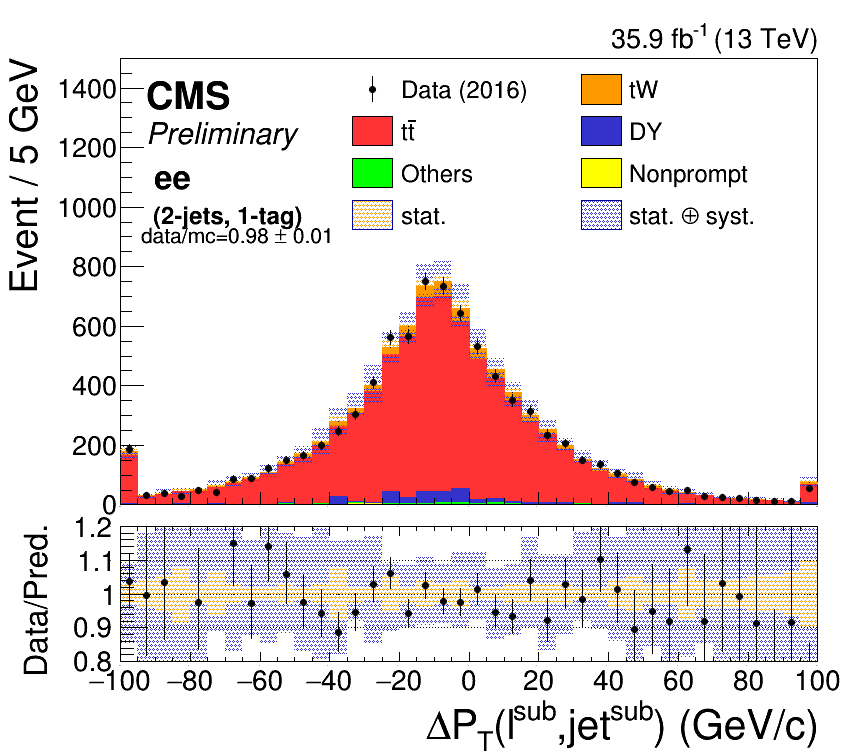
\includegraphics[width=0.4\textwidth]{figures/tW/fig/MVA_input/ee/H_2j1b_dPt_l2_j2.png}&
      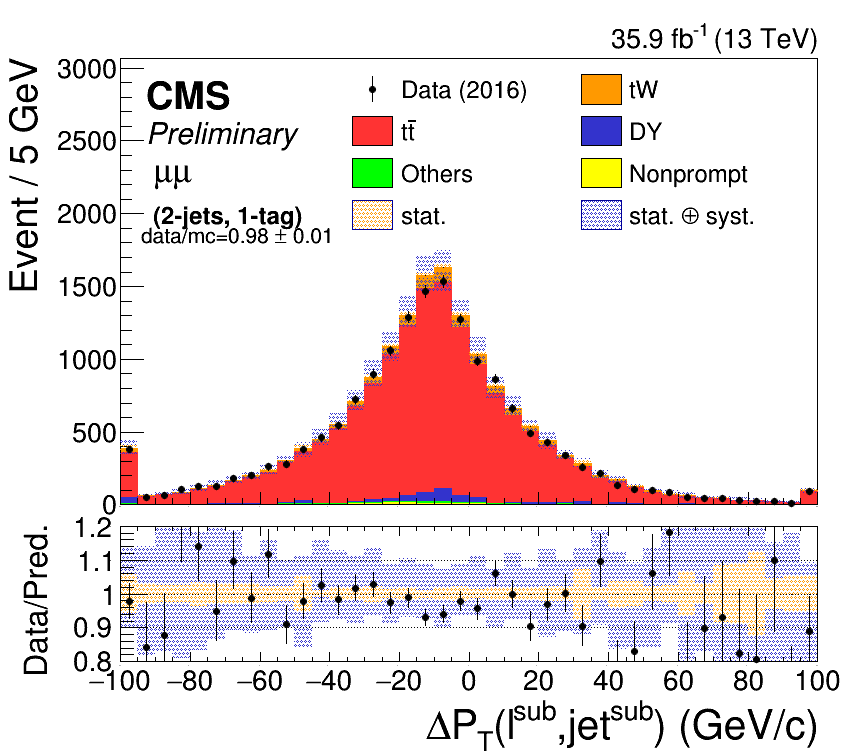
\includegraphics[width=0.4\textwidth]{figures/tW/fig/MVA_input/mumu/H_2j1b_dPt_l2_j2.png}\\
      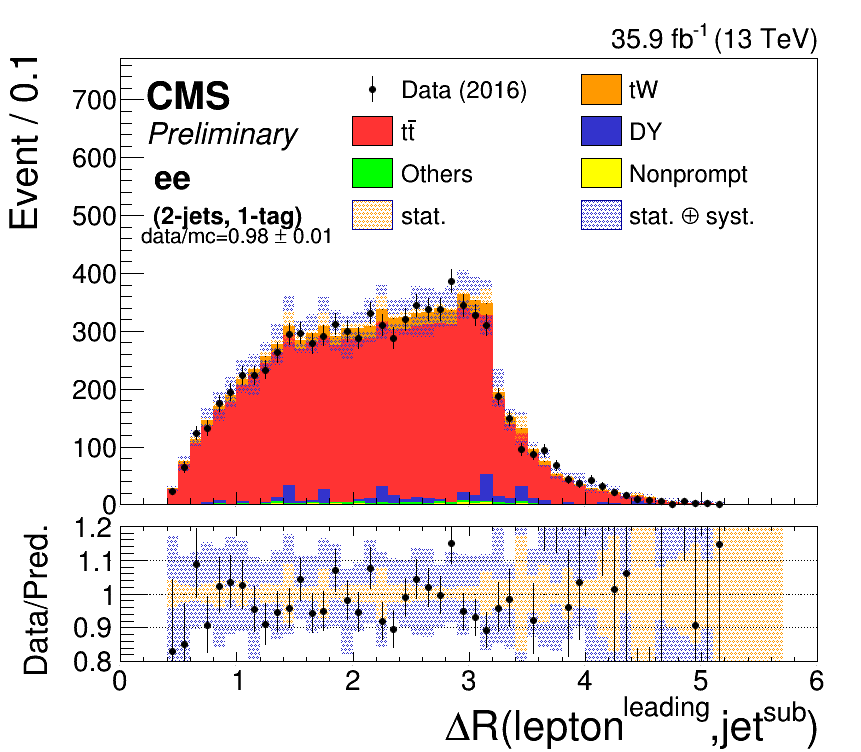
\includegraphics[width=0.4\textwidth]{figures/tW/fig/MVA_input/ee/H_2j1b_dR_l1_j2.png}&
      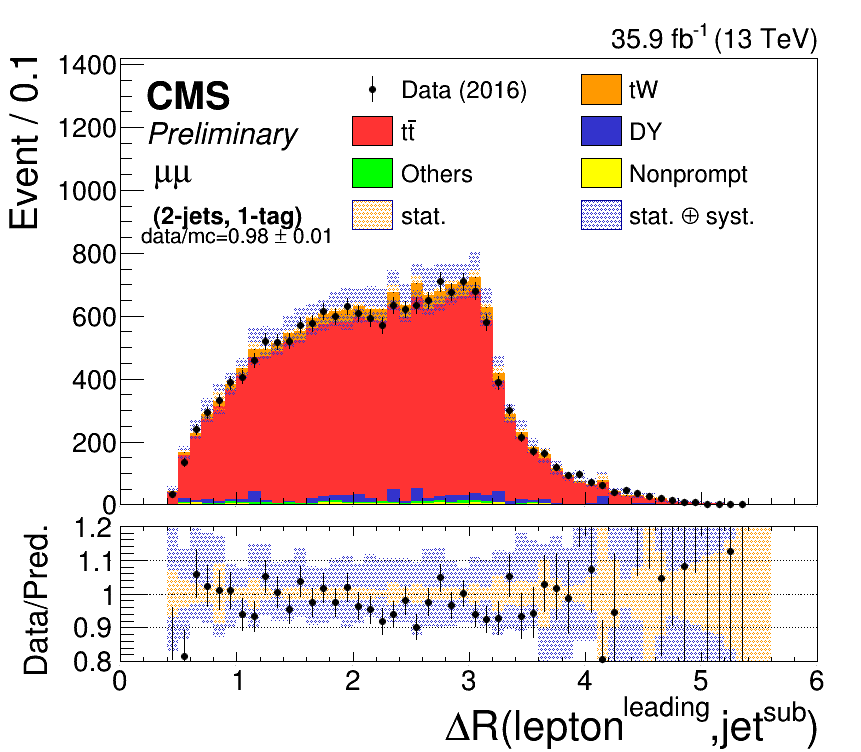
\includegraphics[width=0.4\textwidth]{figures/tW/fig/MVA_input/mumu/H_2j1b_dR_l1_j2.png}\\
      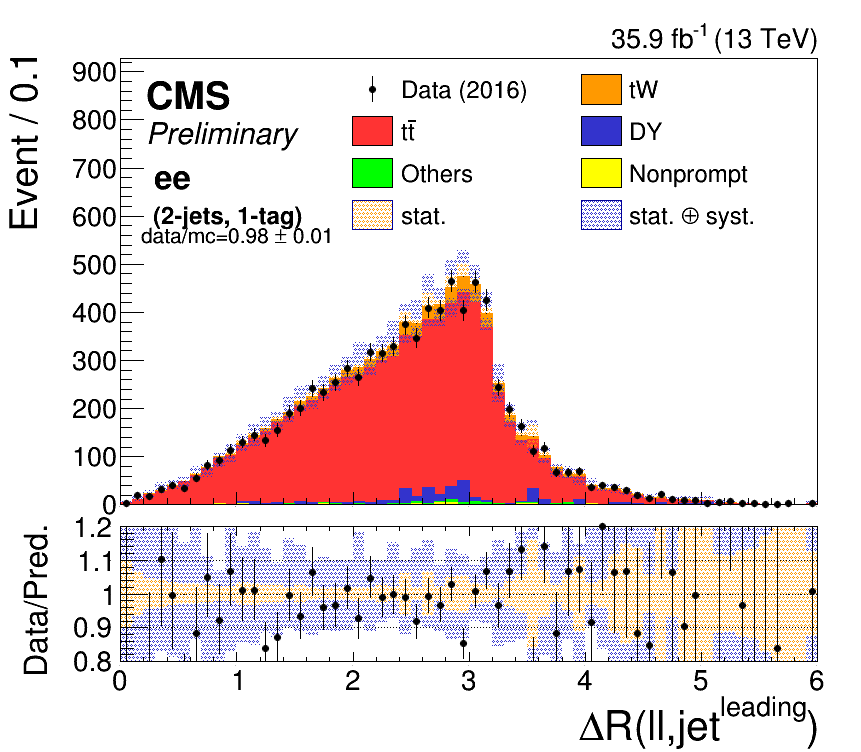
\includegraphics[width=0.4\textwidth]{figures/tW/fig/MVA_input/ee/H_2j1b_dR_ll_j1.png}&
      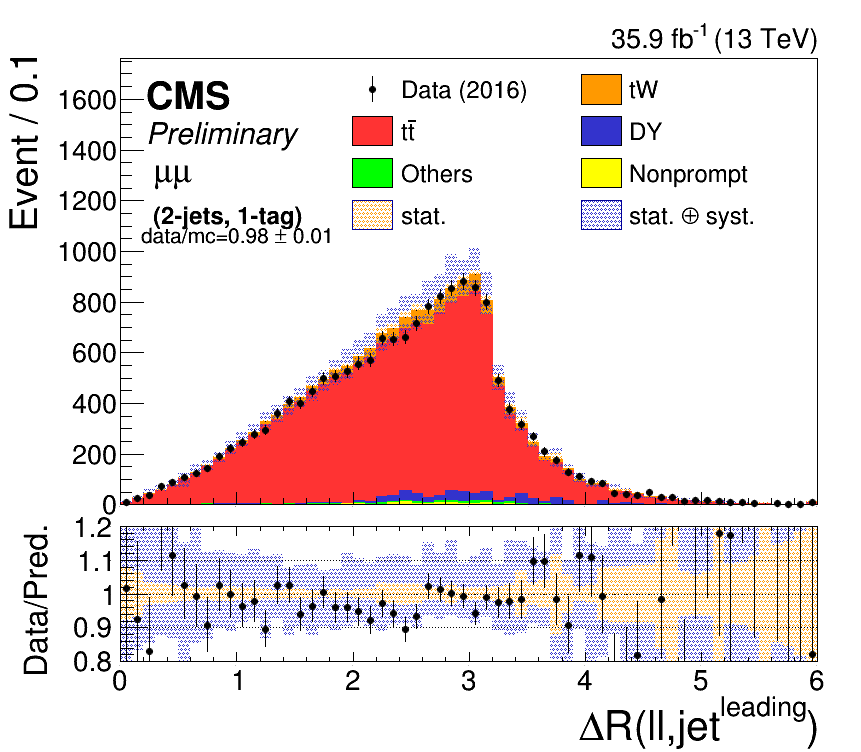
\includegraphics[width=0.4\textwidth]{figures/tW/fig/MVA_input/mumu/H_2j1b_dR_ll_j1.png}\\
    \end{tabular}
    \caption{The distributions of variables used for MVA input for $ee$ (left) and $\mu\mu$ (right) channels for NN$_{21}$.
    \label{fig:MVA_2j1t_1}}
  \end{center}
\end{figure}

\begin{figure}[ht]
  \begin{center}
    \begin{tabular}{ccc}
      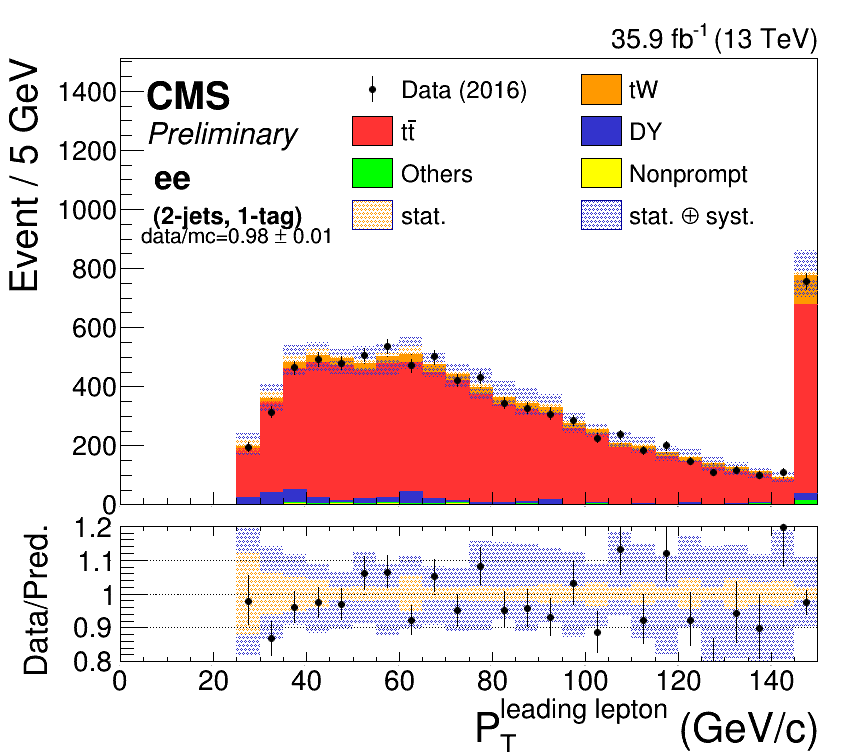
\includegraphics[width=0.4\textwidth]{figures/tW/fig/MVA_input/ee/H_2j1b_l1_pt.png}&
      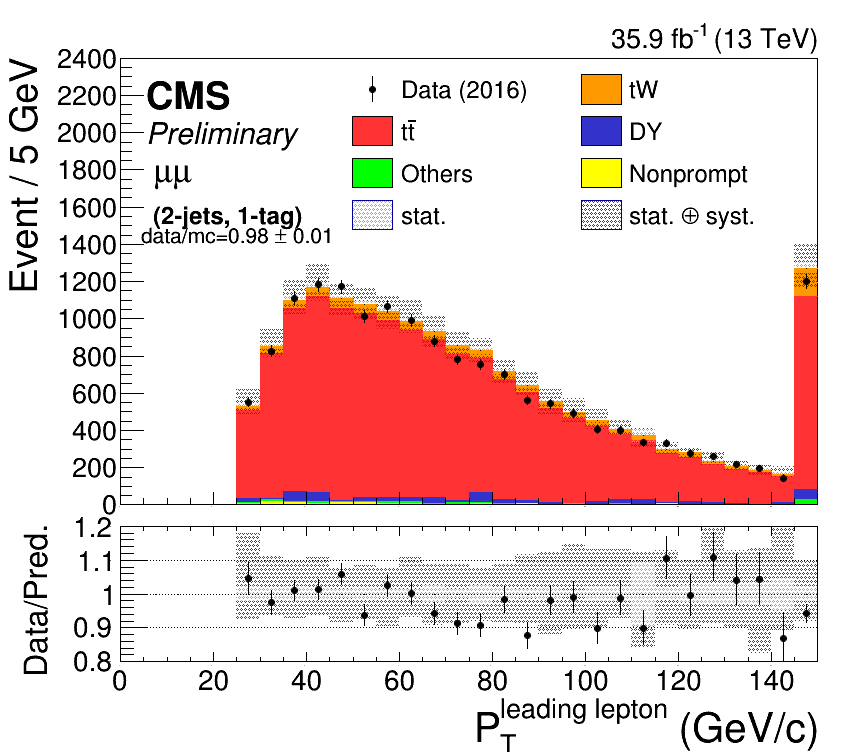
\includegraphics[width=0.4\textwidth]{figures/tW/fig/MVA_input/mumu/H_2j1b_l1_pt.png}\\
      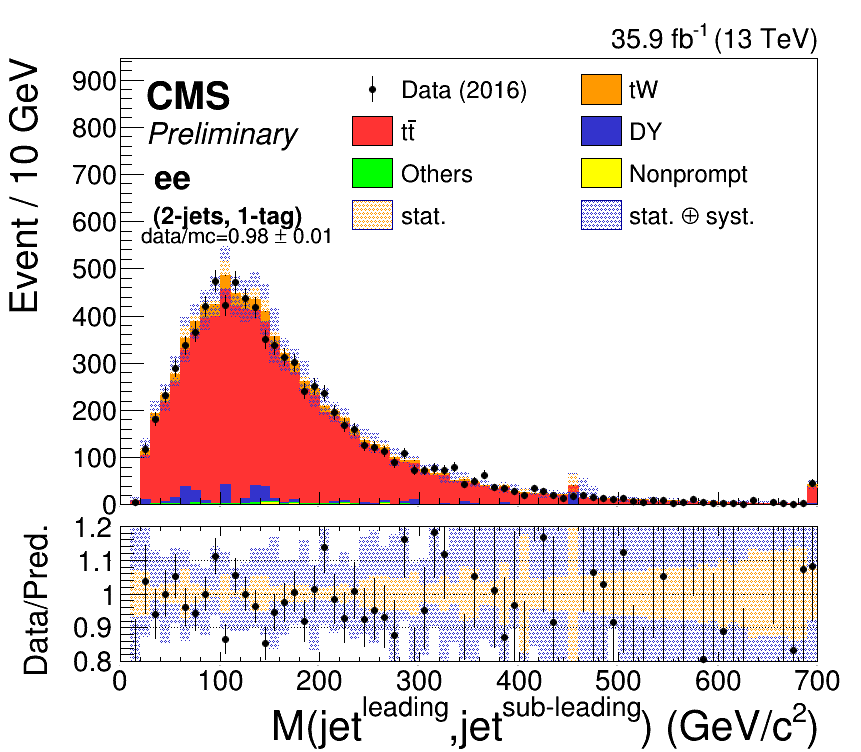
\includegraphics[width=0.4\textwidth]{figures/tW/fig/MVA_input/ee/H_2j1b_M_j1_j2.png}&
      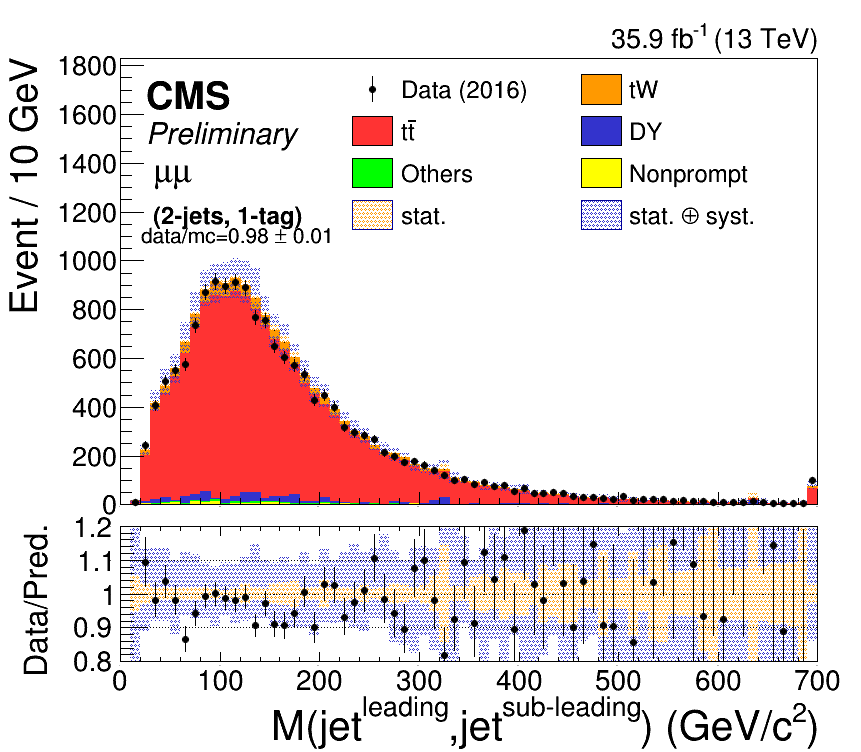
\includegraphics[width=0.4\textwidth]{figures/tW/fig/MVA_input/mumu/H_2j1b_M_j1_j2.png}\\
      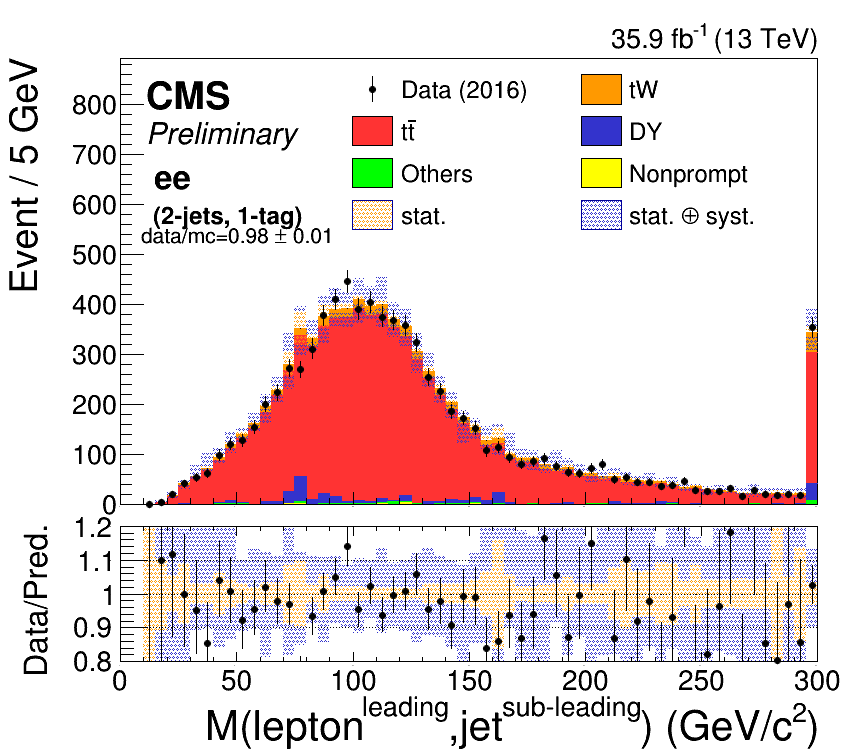
\includegraphics[width=0.4\textwidth]{figures/tW/fig/MVA_input/ee/H_2j1b_M_l1_j2.png}&
      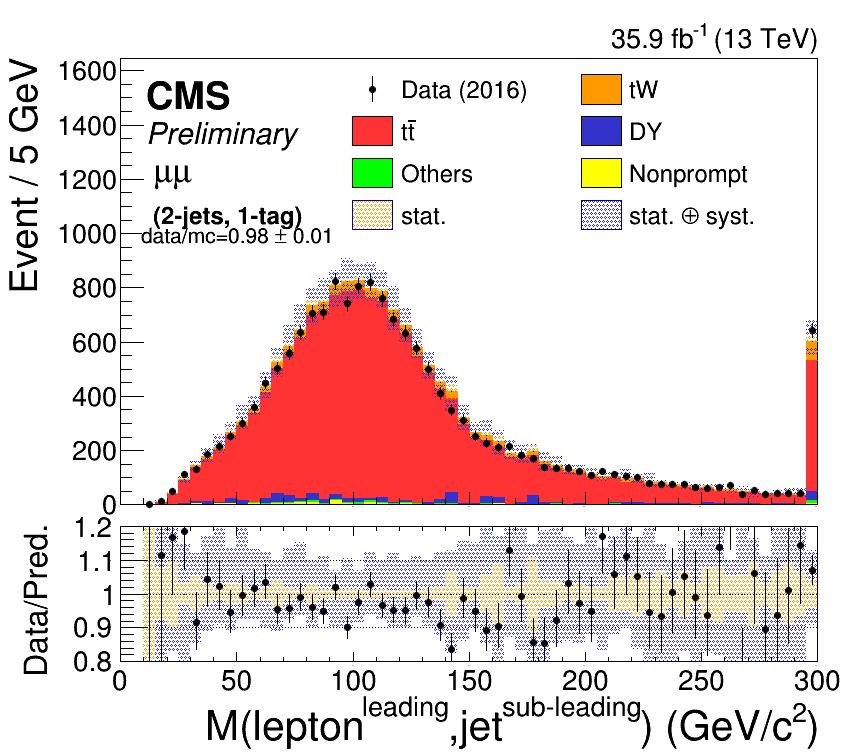
\includegraphics[width=0.4\textwidth]{figures/tW/fig/MVA_input/mumu/H_2j1b_M_l1_j2.png}\\
      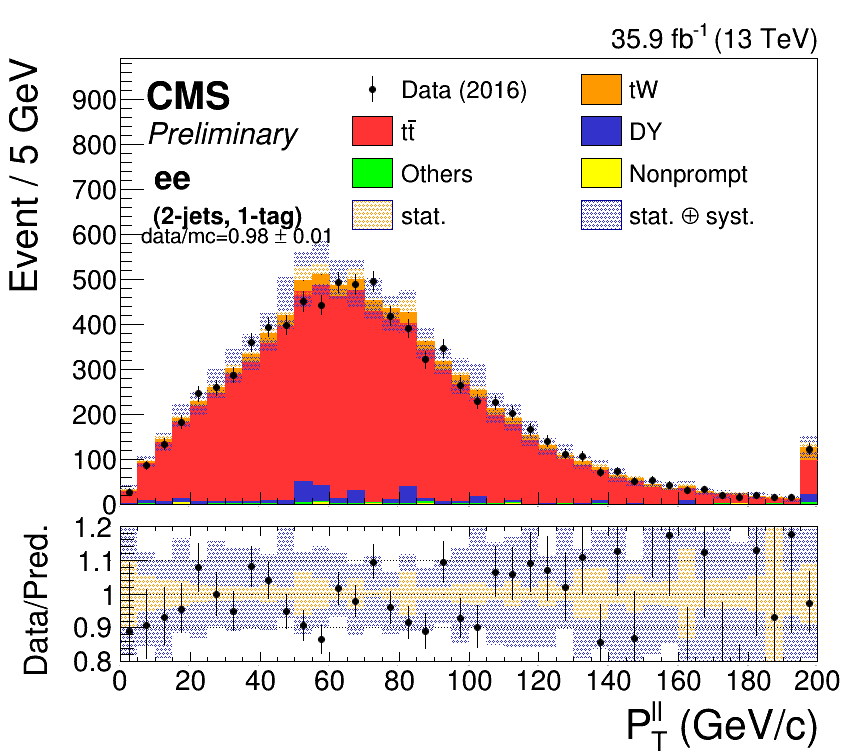
\includegraphics[width=0.4\textwidth]{figures/tW/fig/MVA_input/ee/H_2j1b_Ptll.png}&
      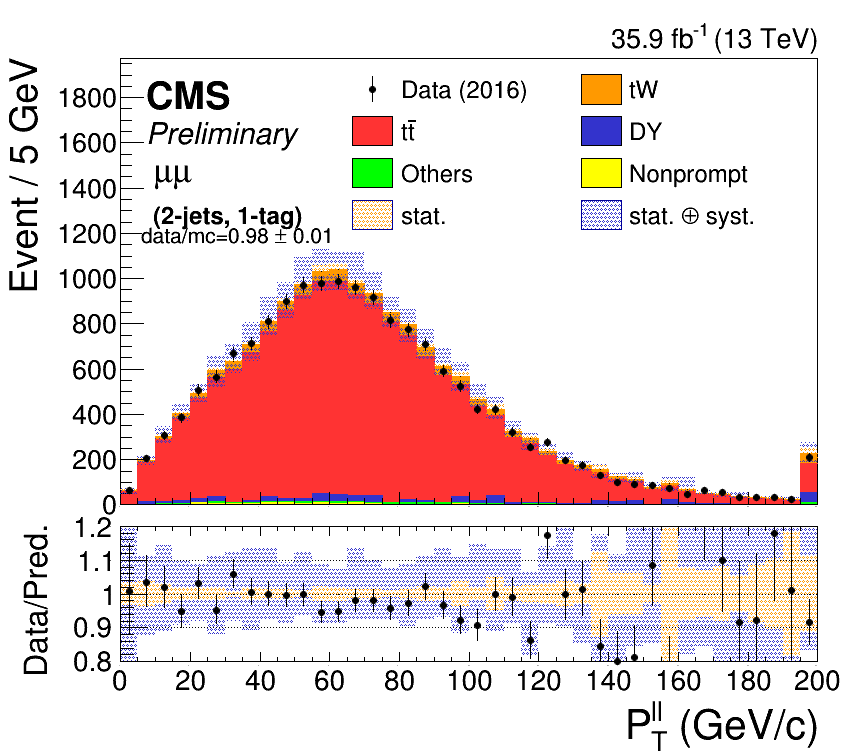
\includegraphics[width=0.4\textwidth]{figures/tW/fig/MVA_input/mumu/H_2j1b_Ptll.png}\\
    \end{tabular}
    \caption{The distributions of variables used for MVA input for $ee$ (left) and $\mu\mu$ (right) channels for NN$_{21}$.
    \label{fig:MVA_2j1t_2}}
  \end{center}
\end{figure}





\begin{figure}[ht]
  \begin{center}
    \begin{tabular}{ccc}
      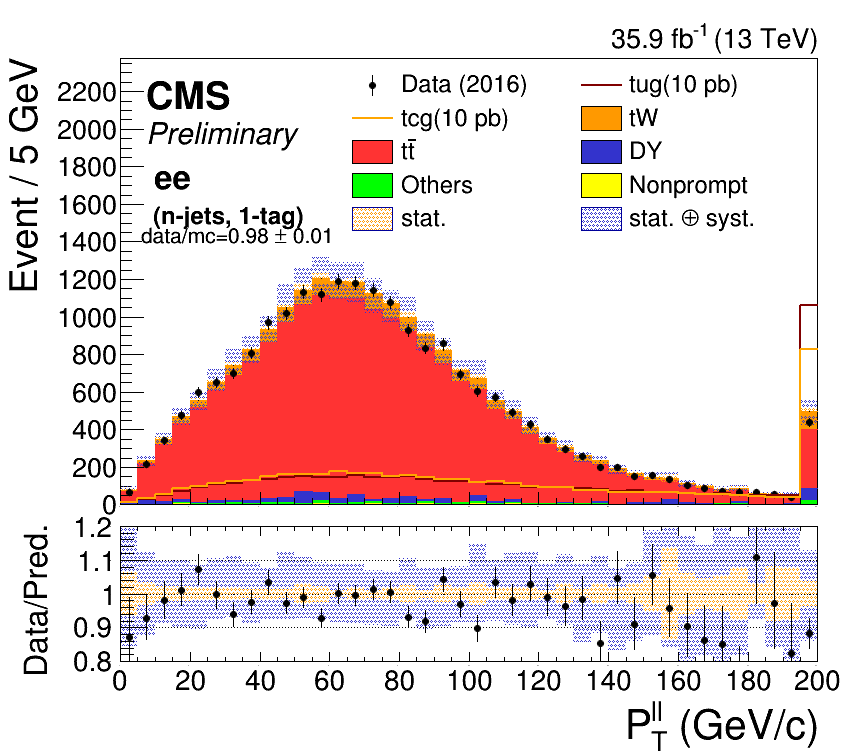
\includegraphics[width=0.4\textwidth]{figures/tW/fig/FCNC_MVA_input/ee/H_BSM_xj1b_Ptll.png}&
      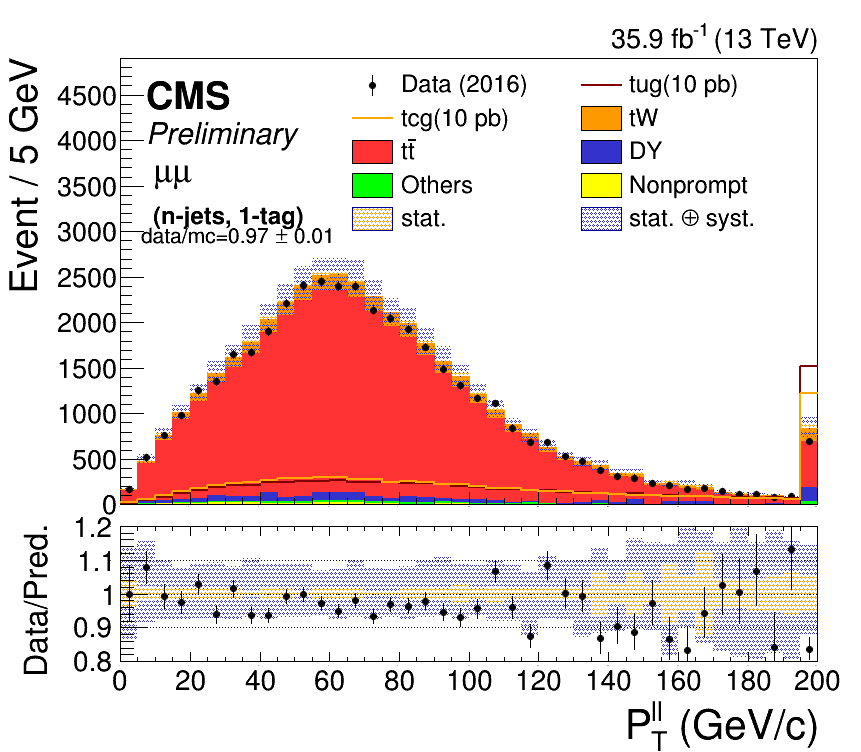
\includegraphics[width=0.4\textwidth]{figures/tW/fig/FCNC_MVA_input/mumu/H_BSM_xj1b_Ptll.png}\\
    \end{tabular}
    \caption{The distributions of variables used for MVA input for FCNC study for $ee$ (left) and $\mu\mu$ (right) channels for NN$_{\text{FCNC}}$.
    \label{fig:MVA_FCNC_1j1t_1}}
  \end{center}
\end{figure}

\begin{figure}[ht]
  \begin{center}
    \begin{tabular}{ccc}
      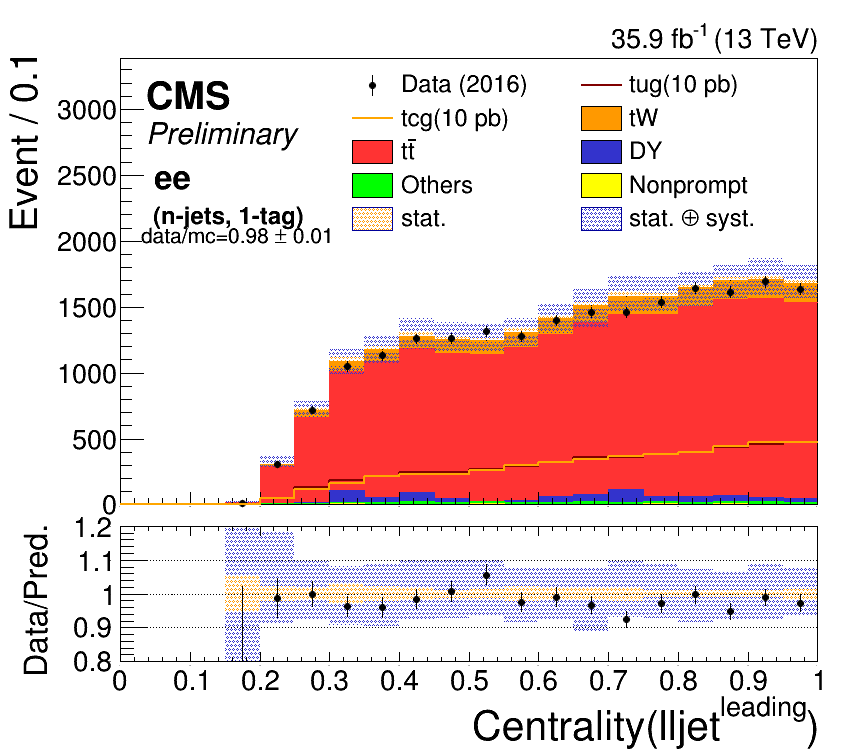
\includegraphics[width=0.4\textwidth]{figures/tW/fig/FCNC_MVA_input/ee/H_BSM_xj1b_Cl1_j1.png}&
      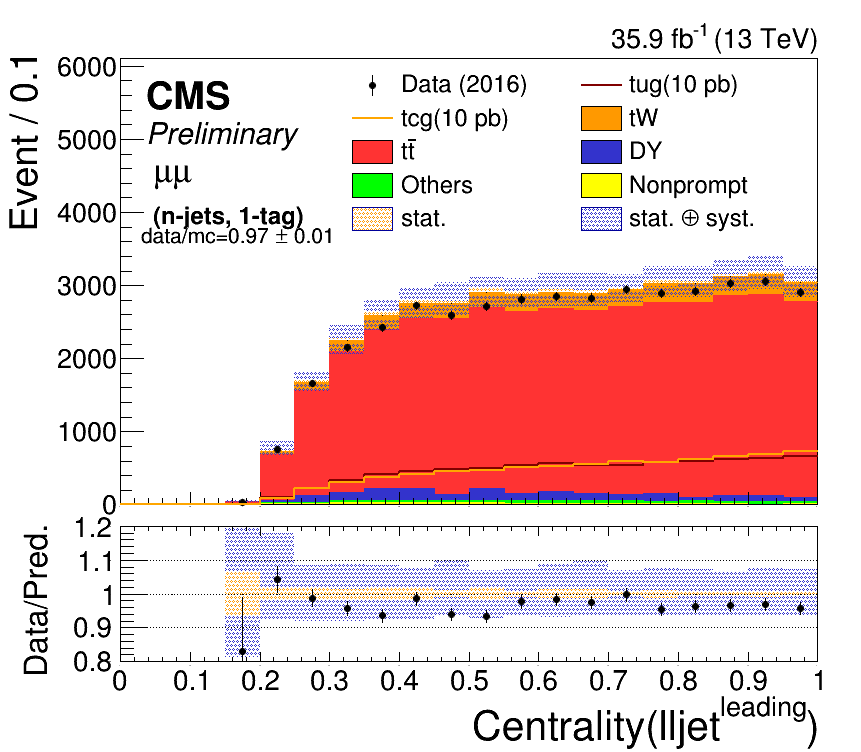
\includegraphics[width=0.4\textwidth]{figures/tW/fig/FCNC_MVA_input/mumu/H_BSM_xj1b_Cl1_j1.png}\\
      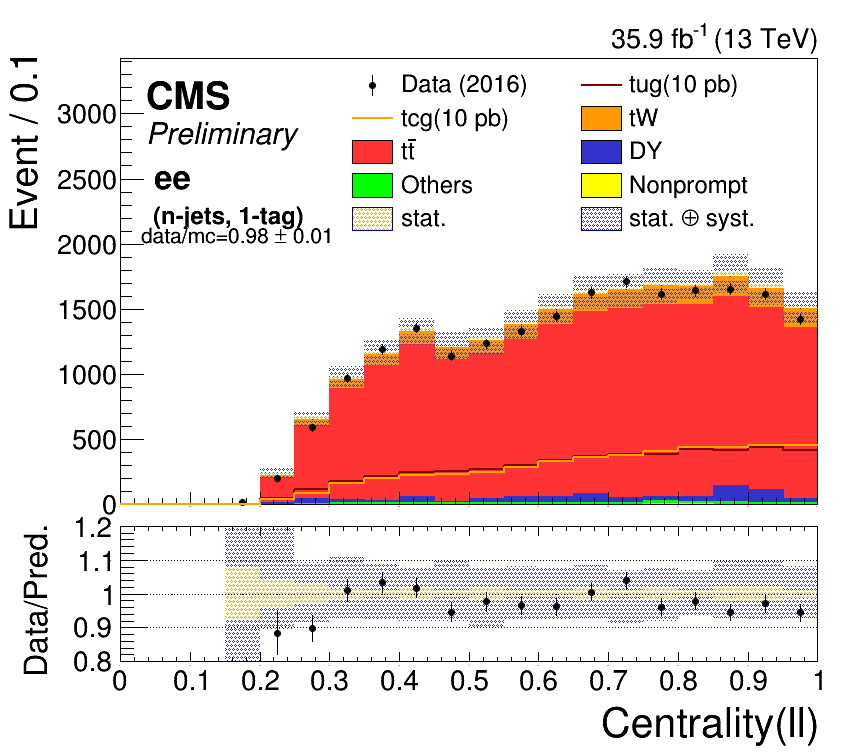
\includegraphics[width=0.4\textwidth]{figures/tW/fig/FCNC_MVA_input/ee/H_BSM_xj1b_Cll.png}&
      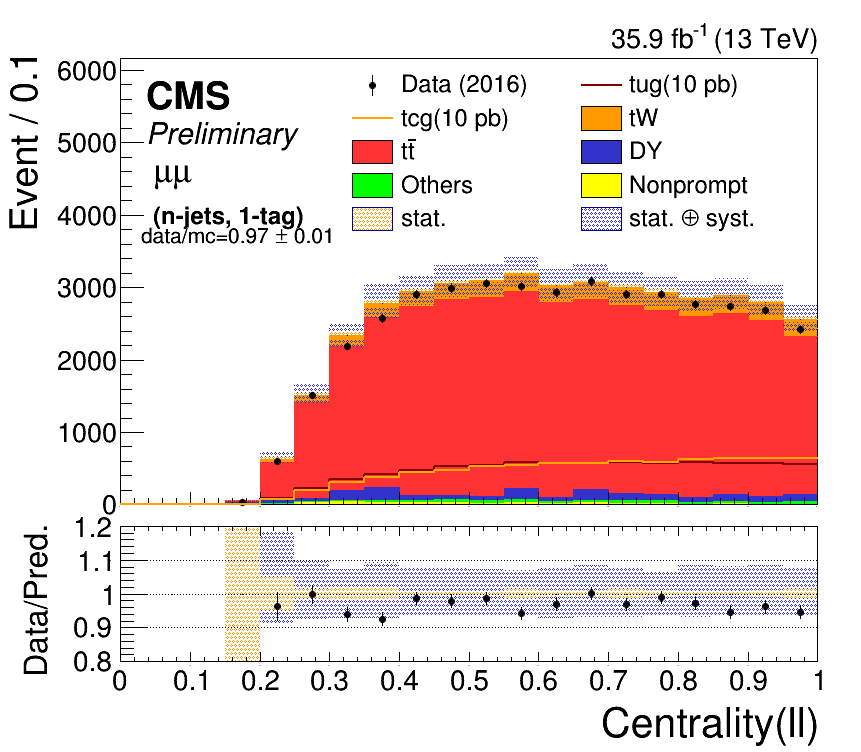
\includegraphics[width=0.4\textwidth]{figures/tW/fig/FCNC_MVA_input/mumu/H_BSM_xj1b_Cll.png}\\
      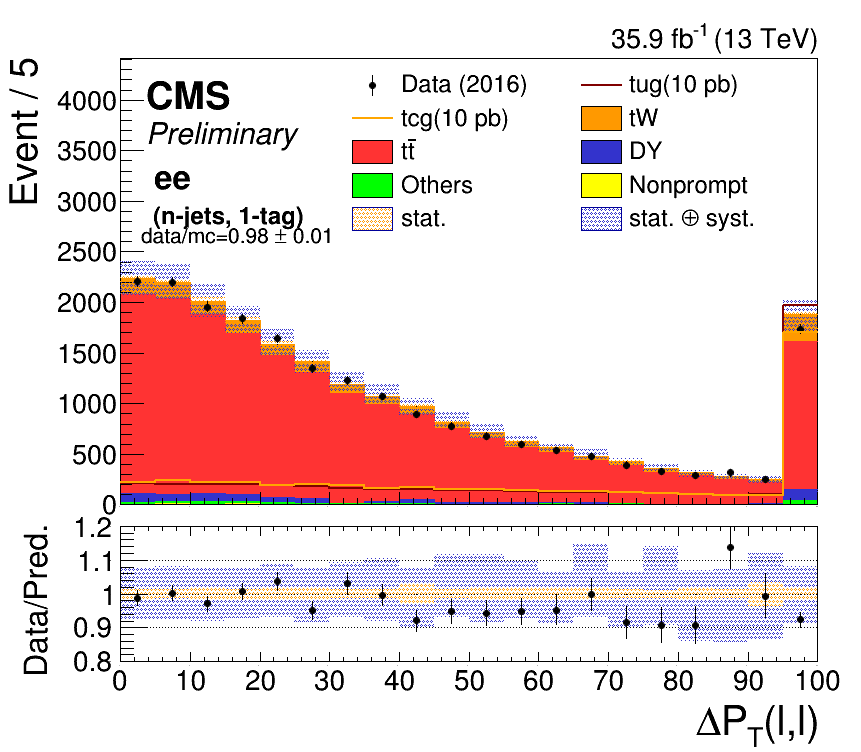
\includegraphics[width=0.4\textwidth]{figures/tW/fig/FCNC_MVA_input/ee/H_BSM_xj1b_dPt_l1_l2.png}&
      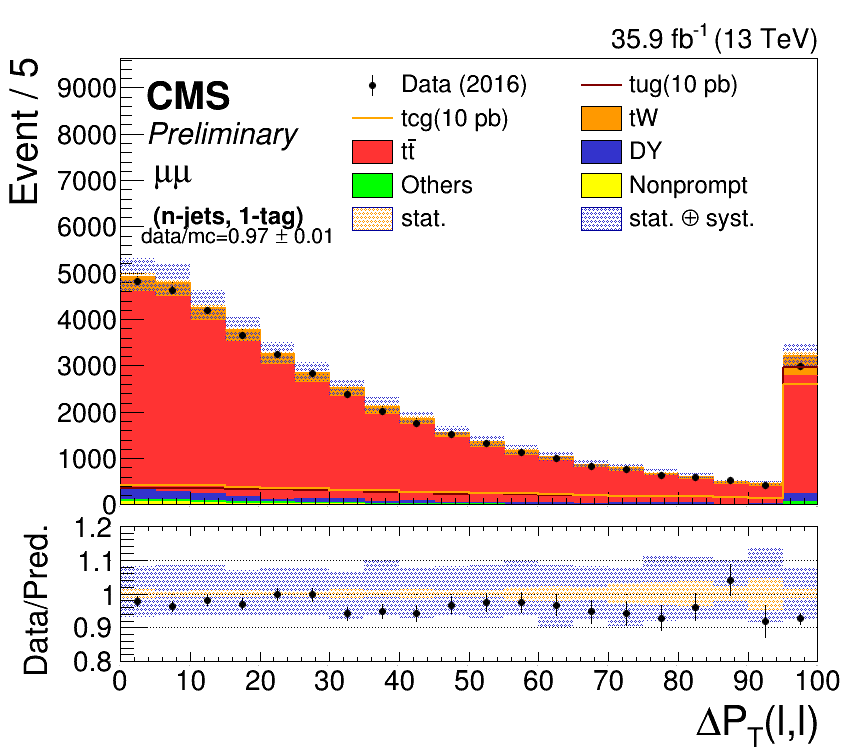
\includegraphics[width=0.4\textwidth]{figures/tW/fig/FCNC_MVA_input/mumu/H_BSM_xj1b_dPt_l1_l2.png}\\
      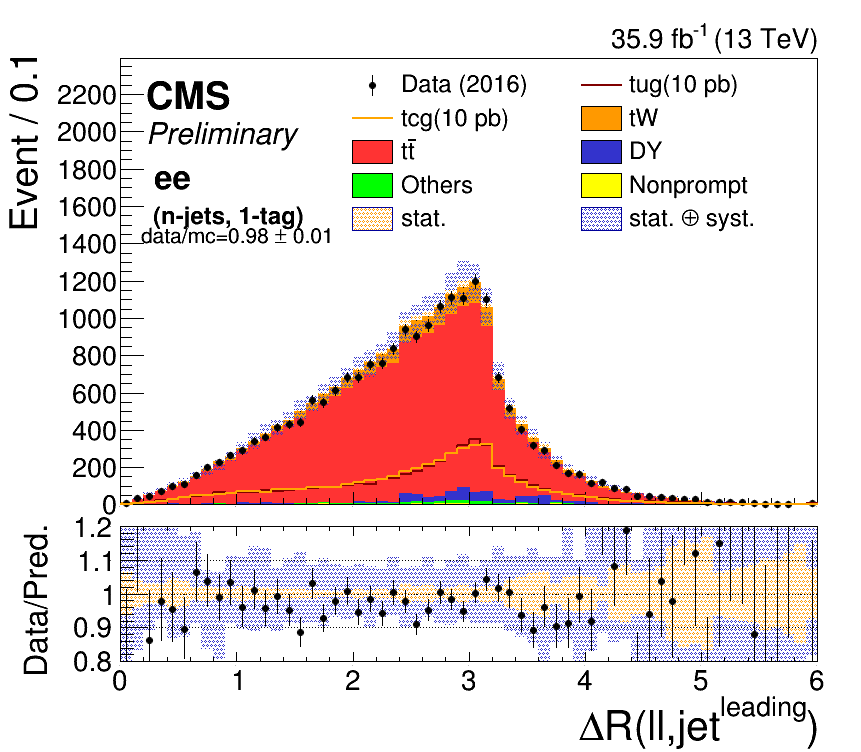
\includegraphics[width=0.4\textwidth]{figures/tW/fig/FCNC_MVA_input/ee/H_BSM_xj1b_dR_ll_j1.png}&
      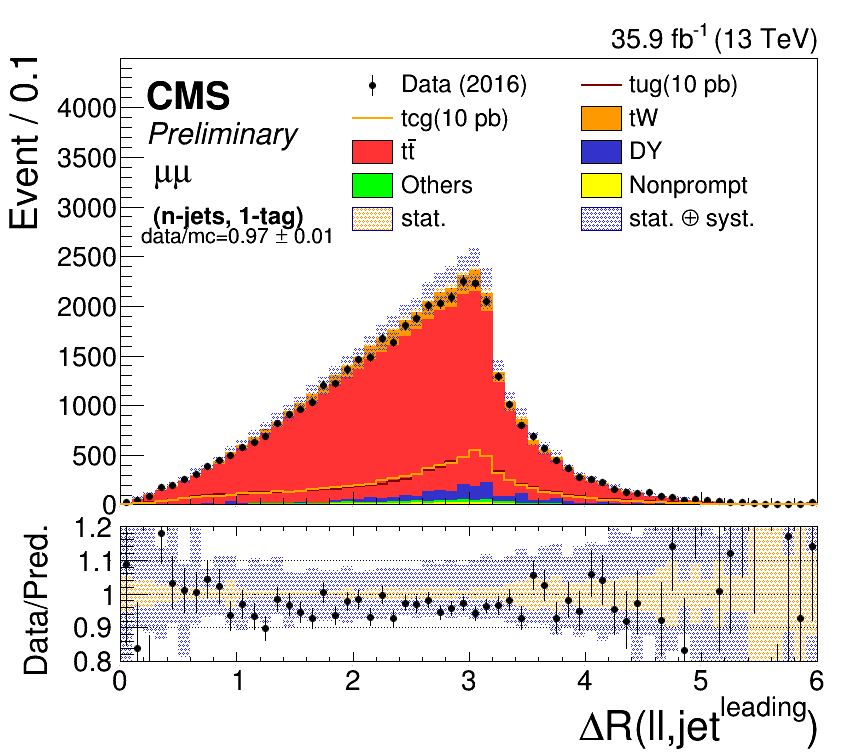
\includegraphics[width=0.4\textwidth]{figures/tW/fig/FCNC_MVA_input/mumu/H_BSM_xj1b_dR_ll_j1.png}\\
    \end{tabular}
    \caption{The distributions of variables used for MVA input for FCNC study for $ee$ (left) and $\mu\mu$ (right) channels for NN$_{\text{FCNC}}$.
    \label{fig:MVA_FCNC_1j1t_2}}
  \end{center}
\end{figure}
\clearpage

\begin{figure}[ht]
  \begin{center}
    \begin{tabular}{ccc}
      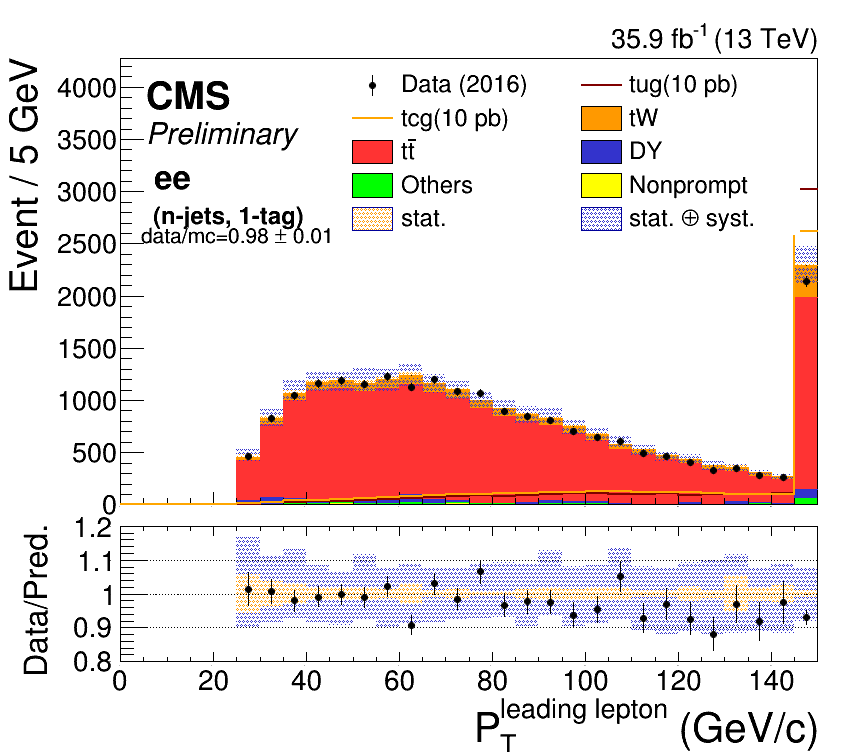
\includegraphics[width=0.4\textwidth]{figures/tW/fig/FCNC_MVA_input/ee/H_BSM_xj1b_l1_pt.png}&
      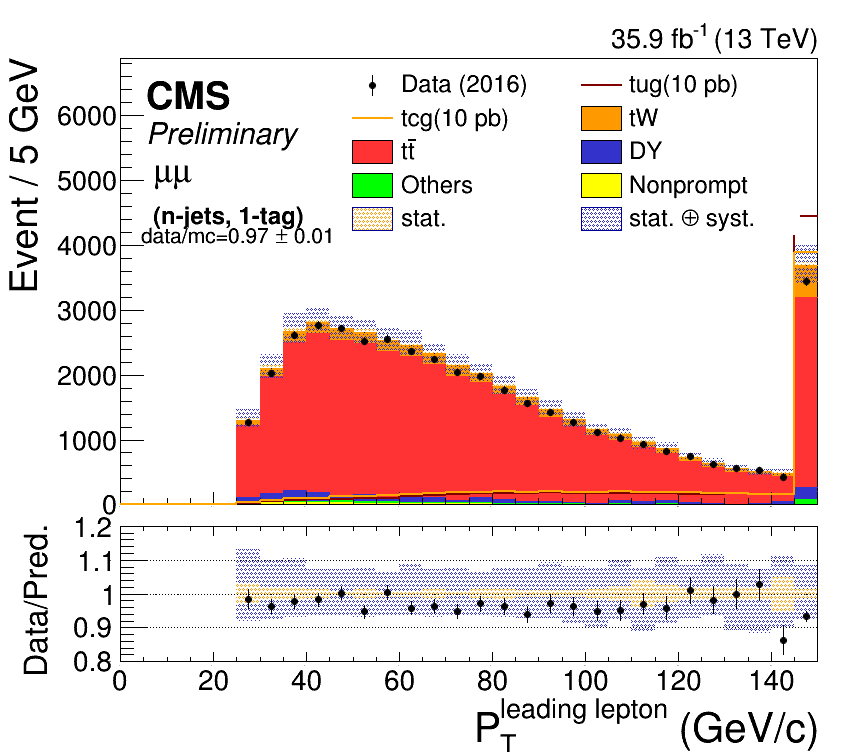
\includegraphics[width=0.4\textwidth]{figures/tW/fig/FCNC_MVA_input/mumu/H_BSM_xj1b_l1_pt.png}\\
      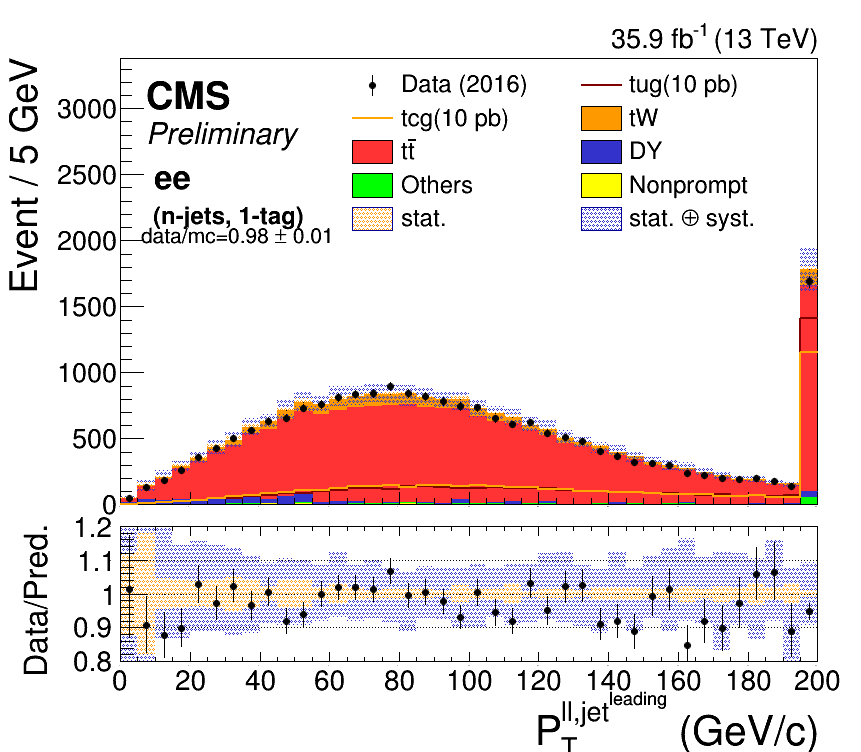
\includegraphics[width=0.4\textwidth]{figures/tW/fig/FCNC_MVA_input/ee/H_BSM_xj1b_ll_j1_pt.png}&
      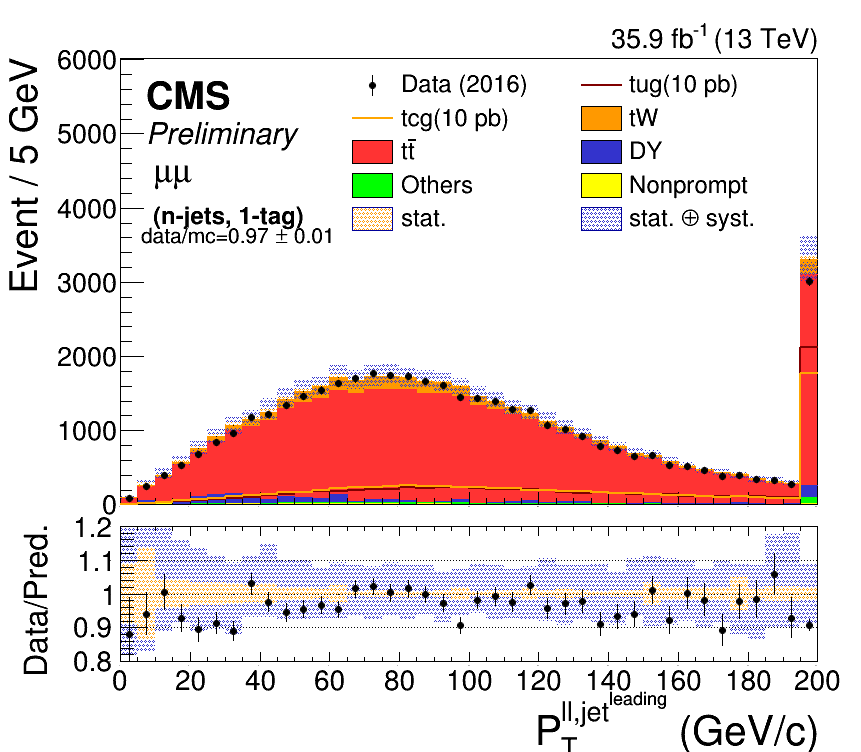
\includegraphics[width=0.4\textwidth]{figures/tW/fig/FCNC_MVA_input/mumu/H_BSM_xj1b_ll_j1_pt.png}\\
      \includegraphics[width=0.4\textwidth]{figures/tW/fig/FCNC_MVA_input/ee/H_BSM_xj1b_M_l2_j1.png}&
      \includegraphics[width=0.4\textwidth]{figures/tW/fig/FCNC_MVA_input/mumu/H_BSM_xj1b_M_l2_j1.png}\\
      \includegraphics[width=0.4\textwidth]{figures/tW/fig/FCNC_MVA_input/ee/H_BSM_xj1b_Mll.png}&
      \includegraphics[width=0.4\textwidth]{figures/tW/fig/FCNC_MVA_input/mumu/H_BSM_xj1b_Mll.png}\\
    \end{tabular}
    \caption{The distributions of variables used for MVA input for FCNC study for $ee$ (left), $e\mu$ (middle) and $\mu\mu$ (right) channels for NN$_{\text{FCNC}}$.
    \label{fig:MVA_FCNC_1j1t_3}}
  \end{center}
\end{figure}

